\RequirePackage{fix-cm}
\documentclass[preprint,12pt,authoryear]{elsarticle}

%% Use the option review to obtain double line spacing
%% \documentclass[authoryear,preprint,review,12pt]{elsarticle}

\usepackage{booktabs}
\usepackage{tabularx}
\usepackage{array}
\usepackage{caption}
\captionsetup[table]{skip=8pt}
\usepackage{microtype}
\emergencystretch=1em
 
\providecommand{\code}[1]{\texttt{#1}}

%% The amssymb package provides various useful mathematical symbols
\usepackage{amssymb}
%% The amsmath package provides various useful equation environments.
\usepackage{amsmath}
%% The amsthm package provides extended theorem environments
%% \usepackage{amsthm}

%% The lineno packages adds line numbers. Start line numbering with
%% \begin{linenumbers}, end it with \end{linenumbers}. Or switch it on
%% for the whole article with \linenumbers.
%% \usepackage{lineno}
\usepackage[colorlinks=true,allcolors=blue]{hyperref}
\hypersetup{
    pdftitle={TrustStatAgent: Conformally calibrated release decisions for large language model statistical agents},
    pdfauthor={Yifei Gao, Jintian Qian, Jiayi Wang, Zhuang Liu}
}
\journal{Expert Systems with Applications}

\usepackage{tikz}
\usetikzlibrary{positioning}
\usepackage{float}
\usepackage{multirow}
\usepackage{graphicx}
\graphicspath{{../}}
\usepackage{tcolorbox}
\tcbuselibrary{skins,breakable}
\newtcolorbox{promptbox}[1]{%
  enhanced, breakable,
  colback=black!2, colframe=black!55,
  colbacktitle=black!15, coltitle=black,
  title={#1}, fonttitle=\small\bfseries\sffamily,
  fontupper=\small\raggedright\ttfamily,
  boxrule=0.5pt, arc=1.2mm,
  left=2.5mm, right=2.5mm, top=2mm, bottom=2mm,
  before skip=8pt, after skip=8pt}

%% Final submission version: all revision colours print as black
\definecolor{blue}{RGB}{0,0,0}
\definecolor{red}{RGB}{0,0,0}

\begin{document}

\begin{frontmatter}

\title{TrustStatAgent: Conformally calibrated release decisions for large language model statistical agents}

%% Author name
\author[inst1]{Yifei Gao}
\ead{2024211169@stumail.dufe.edu.cn}

\author[inst1]{Jintian Qian}
\ead{qianjintian@stumail.dufe.edu.cn}

\author[inst1]{Jiayi Wang}
\ead{2023211013@stumail.dufe.edu.cn}

\author[inst1]{Zhuang Liu\corref{cor1}}
\ead{liuzhuang@dufe.edu.cn}

\cortext[cor1]{Corresponding author.}

%% Author affiliation
\affiliation[inst1]{organization={Dongbei University of Finance and Economics},%Department and Organization
            city={Dalian},
            postcode={116025},
            state={Liaoning},
            country={China}}

%% Abstract
\begin{abstract}
{\color{blue}
Delegating statistical analysis to large language model (LLM) agents is attractive because the work is repetitive and tool-heavy, but an erroneous result is consumed downstream as a fact, and existing pipelines leave the release decision to the user or to a confidence threshold with no finite-sample guarantee. This paper presents TrustStatAgent: an LLM plans the analysis and routes every computation through statistical tools, conformal calibration turns each candidate into an interval or label set with finite-sample coverage, and a deterministic risk gate releases a result only when its execution checks pass and its calibrated output lies inside the task's acceptance region, referring the rest to human review. On four benchmarks spanning question answering, classification, regression and day-ahead forecasting, the gate cuts the released error rate against unrestricted publication by at least three quarters on most of them, and attains a risk--coverage profile that is the lowest or statistically indistinguishable from the lowest throughout, while every released result carries a 90\% coverage certificate. The gain is not free: part of the workload is referred for review, and the release rate accompanies every reliability figure, so the exchange can be weighed against deployment costs.
}
\end{abstract}

%%Graphical abstract
\begin{graphicalabstract}
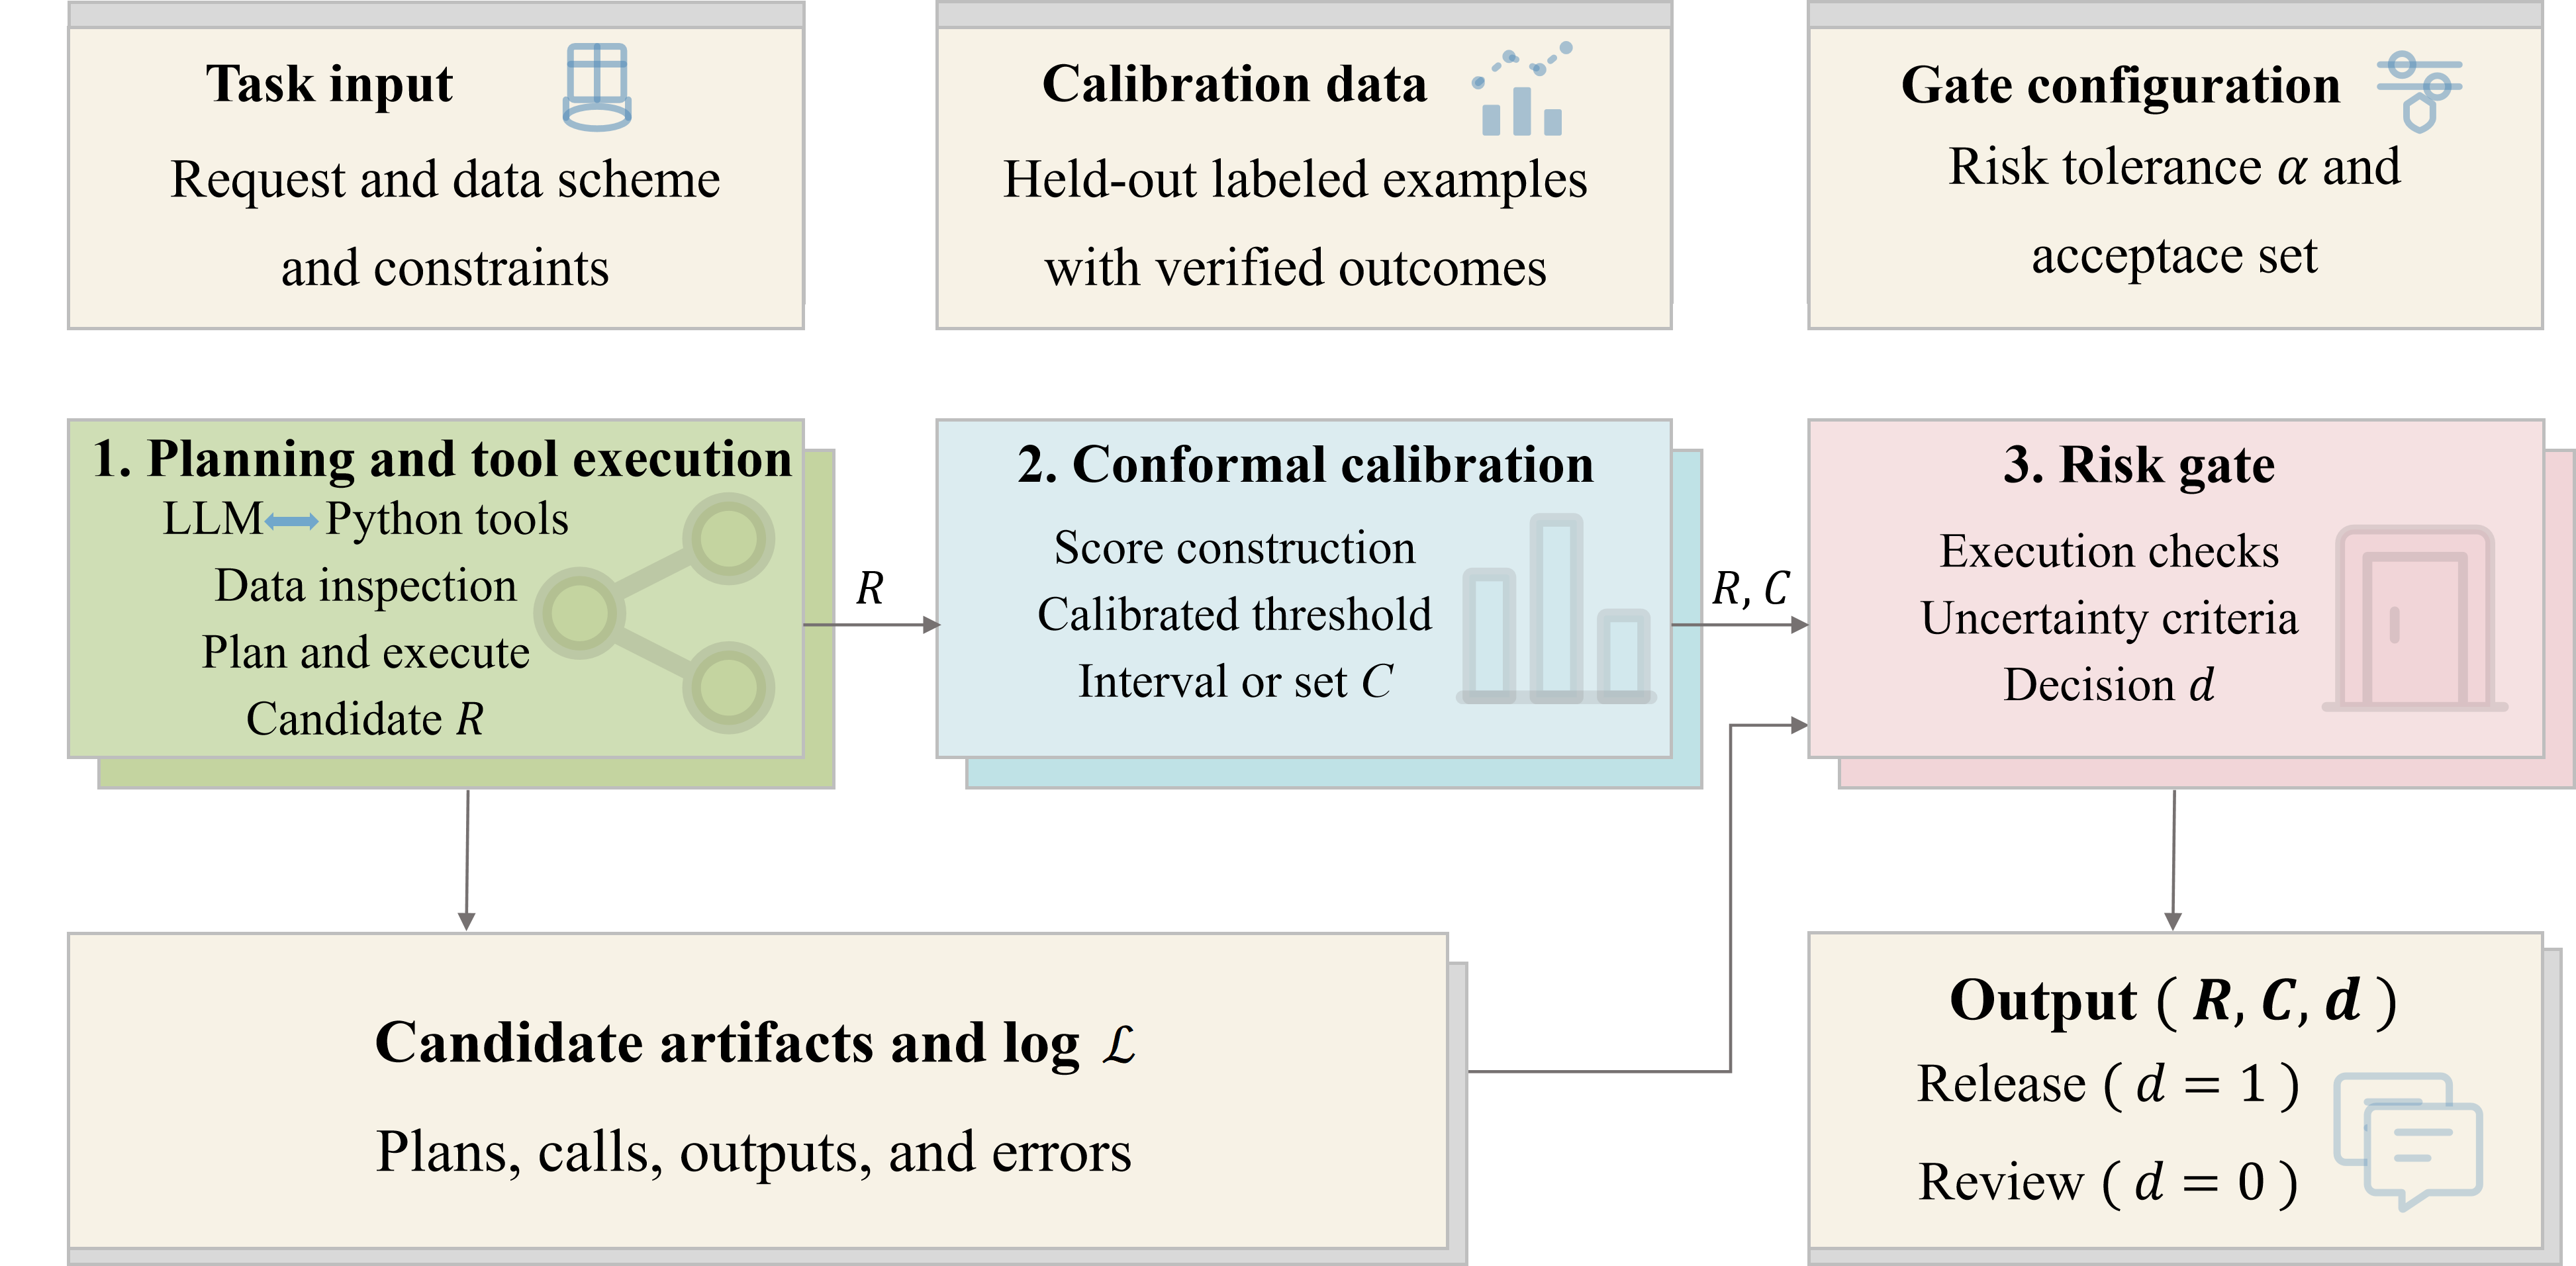
\includegraphics[width=\linewidth]{figures/sci4.png}
\end{graphicalabstract}

%%Research highlights
\begin{highlights}
\item {\color{blue}An LLM statistical agent that decides not only what to compute but what to publish}
\item {\color{blue}The agent plans the analysis and selects methods; tools do all the arithmetic}
\item {\color{blue}Conformal calibration gives every released result a finite-sample coverage guarantee}
\item {\color{blue}A risk gate publishes a result only when execution and uncertainty checks pass}
\item {\color{blue}Released error falls from 43.0\% to \textcolor{red}{10.1}\% on StatQA and \textcolor{red}{to} 1.9\% on Covertype}
\end{highlights}

%% Keywords
\begin{keyword}

Large language model agents \sep Conformal prediction \sep Risk gating
\end{keyword}

\end{frontmatter}

\section{Introduction}
\label{sec1}



Large language models (LLMs) are increasingly deployed as the reasoning core of expert systems. This shift rests on two capabilities. The first is reasoning. Chain-of-thought prompting decomposes a difficult problem into intermediate steps and markedly improves arithmetic and symbolic inference~\citep{wei2022chain}, a behaviour that can be triggered without demonstrations~\citep{kojima2022large} and stabilised by sampling and voting~\citep{wang2023self}. The second is acting. ReAct interleaves reasoning traces with calls to external tools~\citep{yao2023react}, and Toolformer shows that the decision of when to invoke an interface can be learned~\citep{schick2023toolformer}.

Statistical analysis is among the domains in which this capability matters most, because the work involved, such as fitting models, selecting estimators and reporting intervals, is repetitive and tool-heavy. Interest in delegating such work to LLM-based data agents has therefore grown rapidly~\citep{sun2026survey}. Systematic evaluation nevertheless indicates that the capability gap remains wide. On StatQA, a benchmark of 11{,}623 statistical-analysis items, the strongest model attains only 64.83\% accuracy, and its errors are dominated by method applicability rather than computation~\citep{zhu2024large}. The bottleneck is therefore not arithmetic, which can be delegated to deterministic tools, but the judgement surrounding it.

That judgement is also where the reliability of LLMs is weakest. LLMs generate content unfaithful to the available evidence~\citep{ji2023survey}, and their confidence signals are poorly calibrated~\citep{guo2017calibration,kadavath2022language}. Within a statistical pipeline such failures are not merely textual. A misspecified model or an interval that does not cover the quantity it claims to cover is consumed downstream as a fact, and the error is silent. An autonomous statistical agent must therefore decide, for each result, whether that result is safe to release.

Making this requirement precise exposes a difficulty. If reliability is measured as the proportion of released results that are correct, an agent that releases nothing attains a perfect score while completing none of the workload. Reliability is therefore informative only when reported jointly with the fraction of tasks the agent publishes. The objective adopted here is accordingly the joint attainment of statistical accuracy and publishing reliability, which raises three questions. Can a tool-restricted agent match uncalibrated baselines on heterogeneous tasks? Can conformal prediction convert its heuristic uncertainty into statements with finite-sample validity? And does a risk gate discriminate publishable from non-publishable results better than a threshold tuned once on validation data?

An uncertainty layer is the first requirement. Confidence scores are model-specific and carry no finite-sample statement about the quantity of interest. Conformal prediction provides one: it is model-agnostic and distribution-free, and it constructs prediction sets with non-asymptotic coverage guarantees that remain valid under a misspecified model~\citep{lei2018distribution,angelopoulos2023gentle}, with recent extensions controlling the expectation of arbitrary monotone losses~\citep{angelopoulos2024conformal}. Conformal methods have accordingly reached natural language processing~\citep{campos2024conformal,wang2024conu,cherian2024large}. What remains missing is their coupling to the execution of the analysis.

A second requirement concerns how uncertainty becomes an action. Selective prediction formalises the trade-off between coverage and risk and allows a model to abstain where a target risk cannot be met~\citep{geifman2017selective}. In conventional deployments, including the baseline used here, the rejection threshold is tuned once on a validation set and then frozen, which provides no guarantee on the test distribution. Deriving it instead from a quantile of calibration scores lets the decision rule inherit that guarantee. Reliability mechanisms for LLM agents have also attracted attention in the expert-systems community~\citep{shi2025mitigating,he2026enhancing}. The present work supplies a statistical guarantee rather than a consensus heuristic, and attaches it to the decision to publish.

To address these issues, this paper proposes TrustStatAgent, a statistical agent that combines three components. The first is an LLM acting as a planning brain: given a task specification and a restricted toolset for data inspection, model fitting and prediction, it identifies the target variable, the candidate inputs and the task type, emits a structured plan, and routes every numerical computation through the tools. Its instructions forbid fabricated results and forbid the model from deciding whether its own output may be released. The second is conformal calibration, which uses the $\lceil (n+1)(1-\alpha)\rceil$-th smallest nonconformity score on a held-out split to turn point forecasts into intervals and probabilistic label sets into prediction sets. The third is a risk gate, which publishes a result only when its conformal output is valid and a deterministic execution check passes, and defers all other cases to human review.

In summary, the main contributions of this paper are as follows:
\begin{itemize}
  \item We formulate the deployment of LLM-based statistical agents as a joint objective of statistical accuracy and publishing reliability, and we make explicit the evaluation trap whereby a reliability-only criterion can be satisfied through excessive abstention.
  \item We propose TrustStatAgent, which couples tool-grounded execution checking with conformally calibrated uncertainty and a conformal risk gate within a single workflow, separating result generation from result release at the architectural level.
  \item We replace the validation-tuned rejection threshold with a conformally calibrated risk gate, and compare the two directly in their ability to discriminate publishable from non-publishable results.
  \item {\color{blue}We evaluate the framework on four heterogeneous statistical tasks, namely statistical question answering on StatQA~\citep{zhu2024large}, seven-class classification on Covertype~\citep{blackard1999comparative}, regression on California Housing~\citep{pace1997sparse} and day-ahead price forecasting on Energy-Charts data~\citep{energycharts2025}, and we isolate the contribution of explicit planning, conformal calibration and risk gating through targeted ablations.}
\end{itemize}

%This paper is organized as follows. Section~2 reviews related work on LLM agents, uncertainty quantification and selective prediction. Section~3 presents the TrustStatAgent framework. Section~4 describes the datasets, baselines and evaluation metrics. Section~5 reports and discusses the experimental results. Section~6 concludes the paper and outlines directions for future work.

\section{Related Work}
\subsection{Large language model agents for statistical analysis}
\label{subsec:statistical_agents}
Large language models (LLMs) offer a new interface for data analysis through natural language. Users can describe an analytical task, and the model can identify relevant variables, organize the required steps,and invoke external tools to perform computations. In this workflow, the LLM interprets the task and plans the analysis, while statistical tools perform numerical computations and execute models. ReAct interleaves reasoning and actions so that models can adjust their task trajectories using external feedback~\citep{yao2023react}.Data Interpreter extends this approach to multistage data analysis by representing task dependencies as a graph and incorporating iterative verification and correction~\citep{hong2025data}.These studies provide a foundation for translating natural language requests into executable workflows.

Statistical analysis imposes explicit constraints on variable definitions, data types, and the applicability of methods. Consequently, a computation that returns successfully does not establish that the analytical choices were appropriate. StatQA evaluates the joint selection of relevant variables and applicable statistical methods and identifies limitations in LLMs' assessment of method applicability~\citep{zhu2024large}. Evaluating a statistical agent therefore requires distinguishing task interpretation, method selection, and tool execution. 

Existing research on tool use provides mechanisms for generating candidate statistical results. Whether these results are suitable for direct use, however, requires further assessment. Conformal inference provides a principled way to supplement point predictions with prediction intervals offering finite-sample marginal coverage under exchangeability~\citep{lei2018distribution}. Methodological choices also warrant scrutiny: independent teams analyzing the same dataset can obtain substantially different results through different analytical workflows~\citep{botvinik2020variability}. Furthermore, selective classification explicitly distinguishes prediction from the decision to accept or reject it, formalizing the trade-off between predictive risk and the proportion of accepted predictions~\citep{elyaniv2010foundations}. Motivated by these considerations, we introduce uncertainty calibration and release decisions as separate stages after tool execution. This design connects task execution with result release and retains the variables, methods, and execution records used to produce each candidate, providing evidence for subsequent decisions.

\subsection{Statistical uncertainty and conformal prediction}
\label{subsec:uncertainty_conformal}
Uncertainty quantification helps connect model predictions with practical decisions. Probabilistic modeling provides a basis for representing and handling uncertainty in models and predictions~\citep{ghahramani2015probabilistic}. For statistical agents, a point prediction or a single candidate answer provides limited information about the strength of the supporting evidence. Moreover, uncalibrated model probabilities may not accurately reflect predictive reliability.

Conformal prediction uses a separate calibration sample to construct prediction intervals or sets and provides finite-sample marginal coverage guarantees under appropriate exchangeability conditions~\citep{angelopoulos2023gentle}. Because conformal prediction can be applied around an existing predictor, it can accommodate outputs from different statistical tools. For regression, conformalized quantile regression (CQR) combines quantile predictions with conformal calibration to produce intervals that reflect variation in uncertainty across observations~\citep{romano2019cqr}. For classification, nonconformity scores can be constructed from the predicted probability of the true class, yielding sets containing one or more candidate classes.

\subsection{Output verification and selective release}
\label{subsec:verification_release}
Trustworthy artificial intelligence encompasses transparency, explainability, fairness, privacy, and reproducibility, among other dimensions. Each system must specify which dimensions it addresses within its intended task~\citep{li2023trustworthy}. Post-generation verification can provide an assessment of model outputs that is separate from the generation process. HaluCheck uses the AutoFactNLI pipeline to decompose generated content, retrieve external evidence, and assess factual relationships, while presenting users with traceable verification results~\citep{heo2025halucheck}. This work highlights the value of inspectable evidence in an evaluation layer: users need to assess whether an output meets predefined requirements alongside any statistical uncertainty representation.

Selective prediction allows a system to abstain on some inputs when the available evidence is insufficient, while considering both prediction risk and the acceptance rate. SelectiveNet integrates prediction with a reject option and examines the trade-off between risk and coverage~\citep{geifman2019selectivenet}. For language model outputs, conformal methods have been used to construct output sets, demonstrating how statistical calibration can contribute to reliability assessment~\citep{quach2024conformal}.

Building on these studies, TrustStatAgent is designed as a calibration and release workflow for heterogeneous statistical tasks. Authorized tools generate candidate results, calibration procedures tailored to the target produce prediction intervals or sets, and execution checks and task requirements determine whether each result can be released automatically.


\section{Methodology}
\label{sec:methodology}
This section describes TrustStatAgent, a workflow for deciding when statistical results can be released automatically. As illustrated in Fig.~\ref{fig:framework}, it combines LLM task planning and statistical tool execution, uncertainty calibration, and a risk gate. We first define the overall framework, then describe these three components in turn.

\begin{figure}[H]
    \centering
    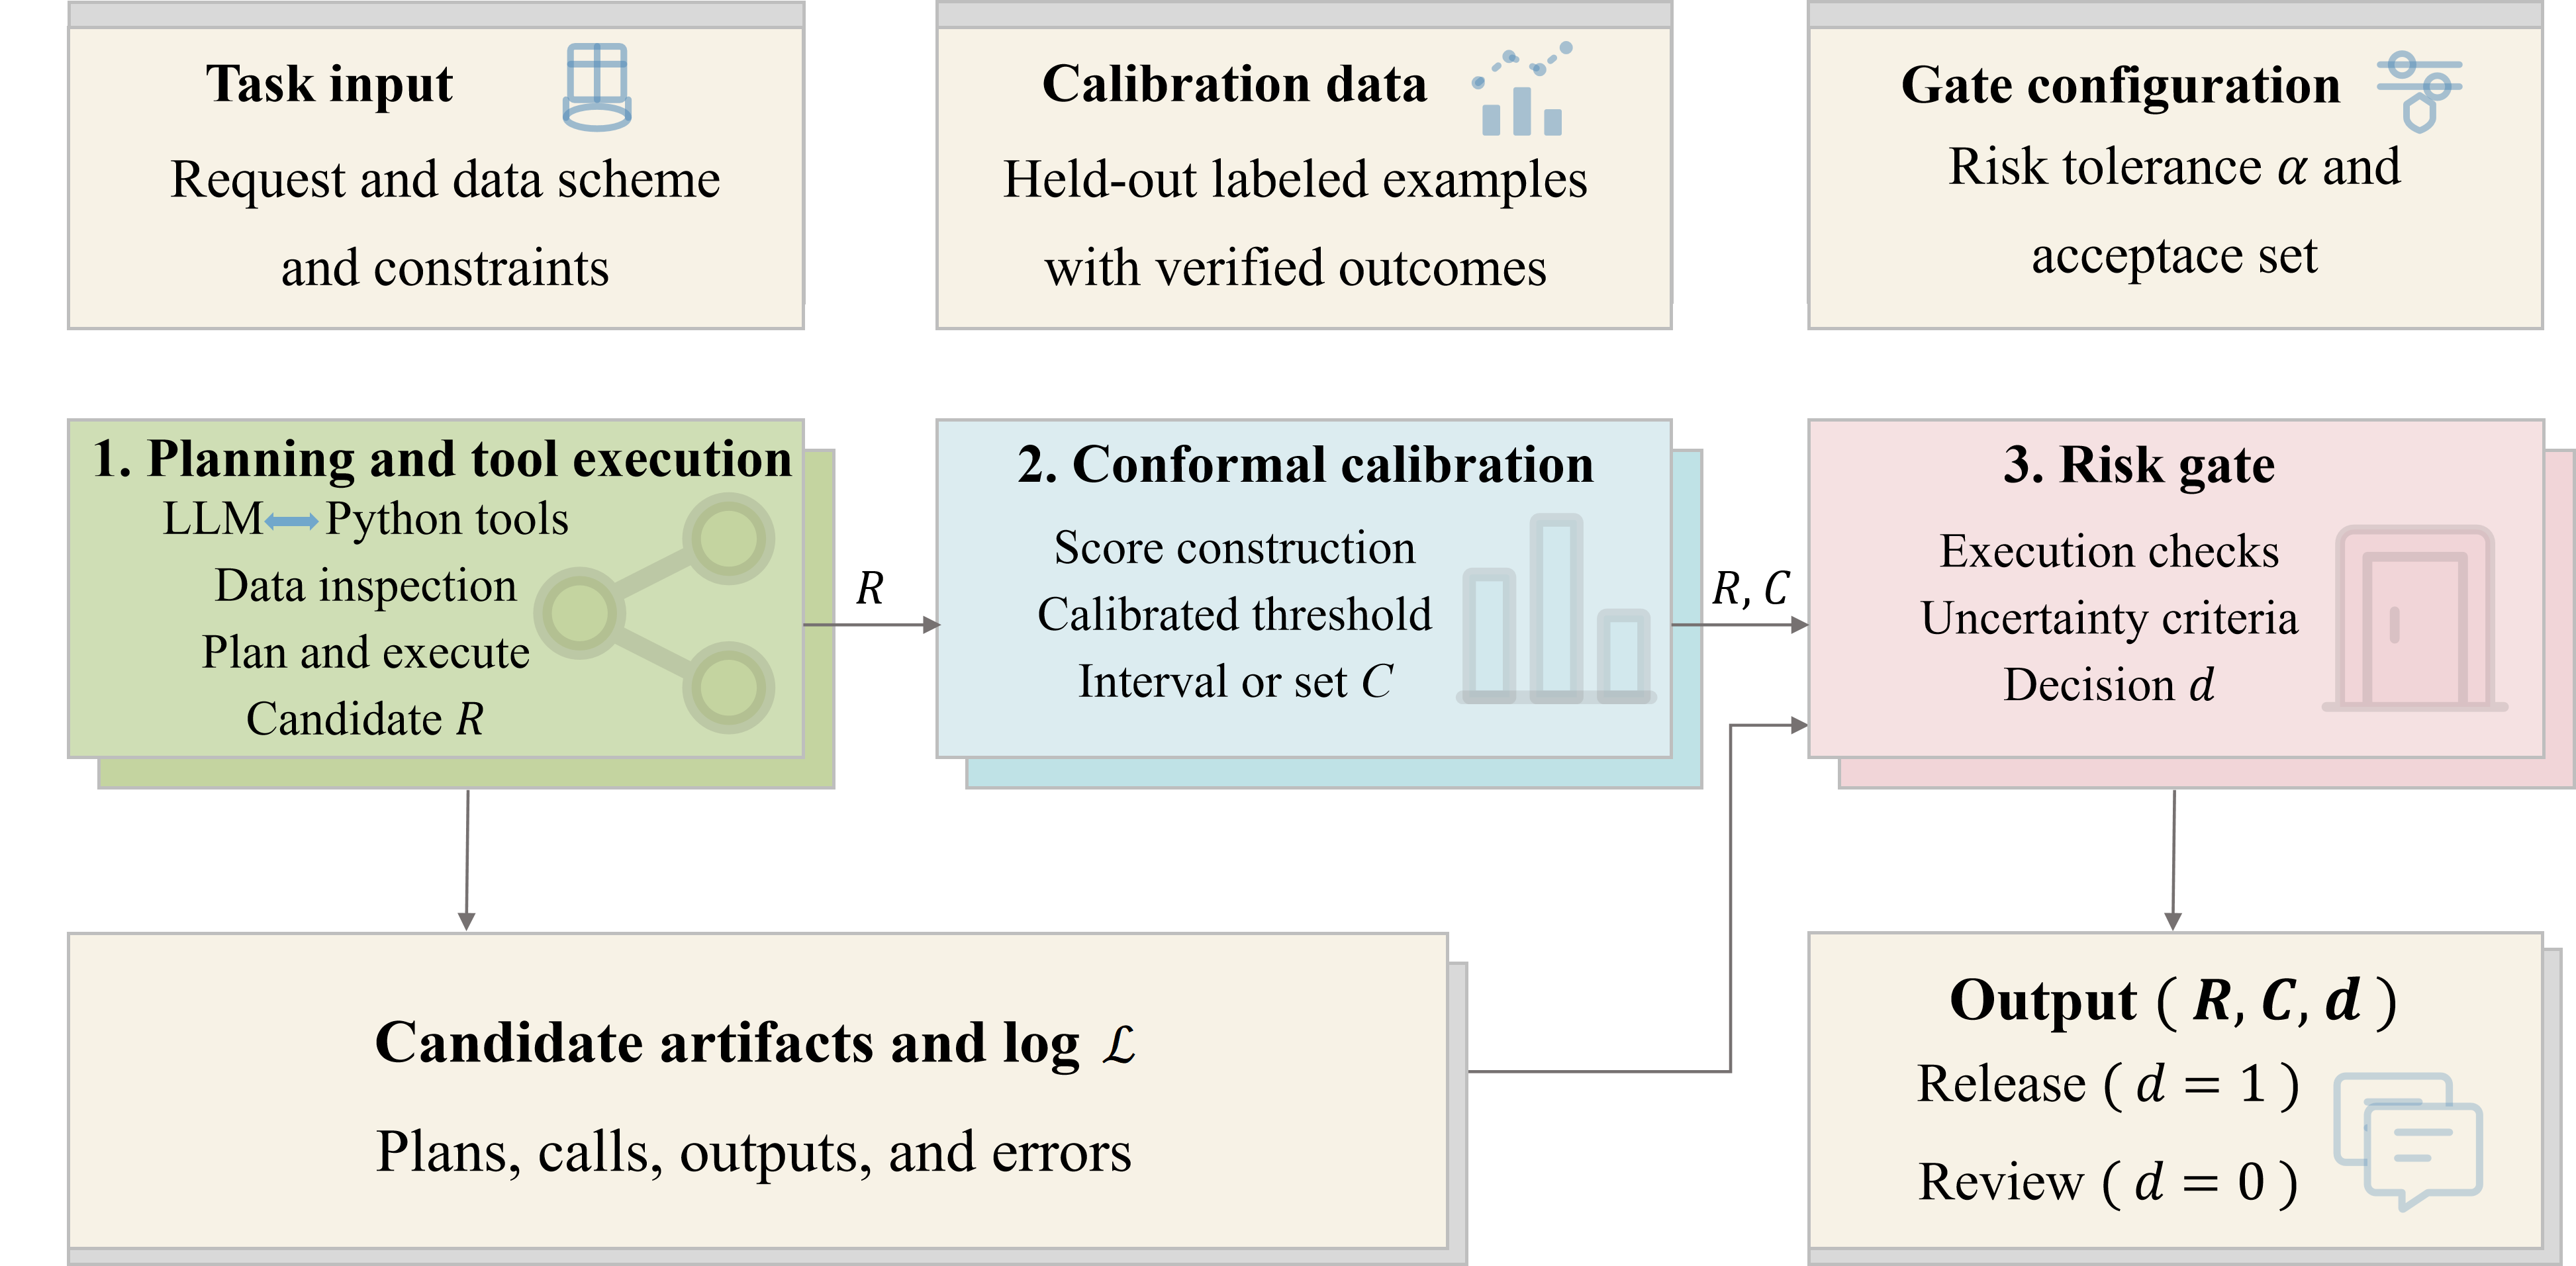
\includegraphics[width=0.92\linewidth]{figures/sci4.png}
    \caption{Overall architecture of TrustStatAgent. Solid arrows indicate task data and execution evidence, while dashed arrows represent calibration and release configurations. Computation, calibration, and gating are fully automated. Human review is required only for execution failures or missing conformal outputs. Calibration labels are isolated from the LLM, and test labels are strictly for evaluation.}
    \label{fig:framework}
\end{figure}

\subsection{Framework and task formulation}
\label{sec:framework}

TrustStatAgent separates task planning and statistical execution, uncertainty calibration, and result release. For a task specification $\mathcal{T}$ and authorized tools $\mathcal{F}$, the first module produces a statistical result $R$ and an execution record $\mathcal{L}$. Calibration then constructs an interval or set $C$ from held-out data, and a deterministic risk gate produces a release decision $g$:
\begin{equation}
    (R,\mathcal{L})=\mathcal{A}_{\theta}(\mathcal{T};\mathcal{F}),\qquad
    C=\mathcal{Q}_{\alpha}(R;\mathcal{D}_{\mathrm{cal}}),\qquad
    g=\mathcal{G}_{\tau}(R,C,\mathcal{L};\Omega),
    \label{eq:framework}
\end{equation}
where $\theta$ denotes the language-model configuration, $\tau$ is the task type, $\alpha$ is the nominal miscoverage level, and $\Omega$ contains task-specific acceptance criteria. The LLM interprets the request and specifies the analysis; authorized programs perform numerical computation and retain execution evidence. A result is released only when its calibrated output and execution status meet the prespecified criteria. {\color{blue}Together, the calibration module and the risk gate form the release layer, which decides what the agent may publish.} We evaluate this design on three predictive tasks and one structured statistical question-answering task, with task-specific implementations described below.

\subsection{Task planning and statistical tool execution}
\label{sec:execution}

The first module translates a natural-language request into an executable analysis. Following the reasoning-and-action pattern of ReAct~\citep{yao2023react}, the LLM receives the user's request, descriptions of the available datasets, and specifications of the permitted statistical tools. It records a structured plan containing the task type, target, selected variables, method, preprocessing, and intended tool sequence. Explicit variable and method selection addresses a documented difficulty in statistical question answering~\citep{zhu2024large}. For numerical tasks, the LLM selects tools for data inspection, model fitting, prediction, or forecasting. Each requested tool call is checked against the permitted tool set and executed by the corresponding statistical procedure. The results are recorded and returned to the LLM to guide subsequent analysis.

{\color{blue}Once produced by this pipeline, the candidates of each predictive task are frozen, so that every release rule evaluated later consumes the identical pool (Section~\ref{sec:evaluation_protocol}). The frozen pool is nevertheless the agent's own work: its method selection yields a random-forest classifier on Covertype, histogram gradient-boosting models for point and quantile predictions on California Housing, and ridge regression selected by chronological cross-validation on Power Price.} In StatQA, the LLM returns the selected columns and methods under an explicit plan, and the benchmark evaluates these analytical choices directly. Its answer correctness follows the benchmark criterion~\citep{zhu2024large}, while a separate TF--IDF logistic-regression scorer supplies the score used for calibration. The scorer is trained on a dedicated split, and reference answers are excluded from its input features.
Figure~\ref{fig:planning_execution} illustrates this
workflow using a house-value prediction request.

\begin{figure}[H]
    \centering
    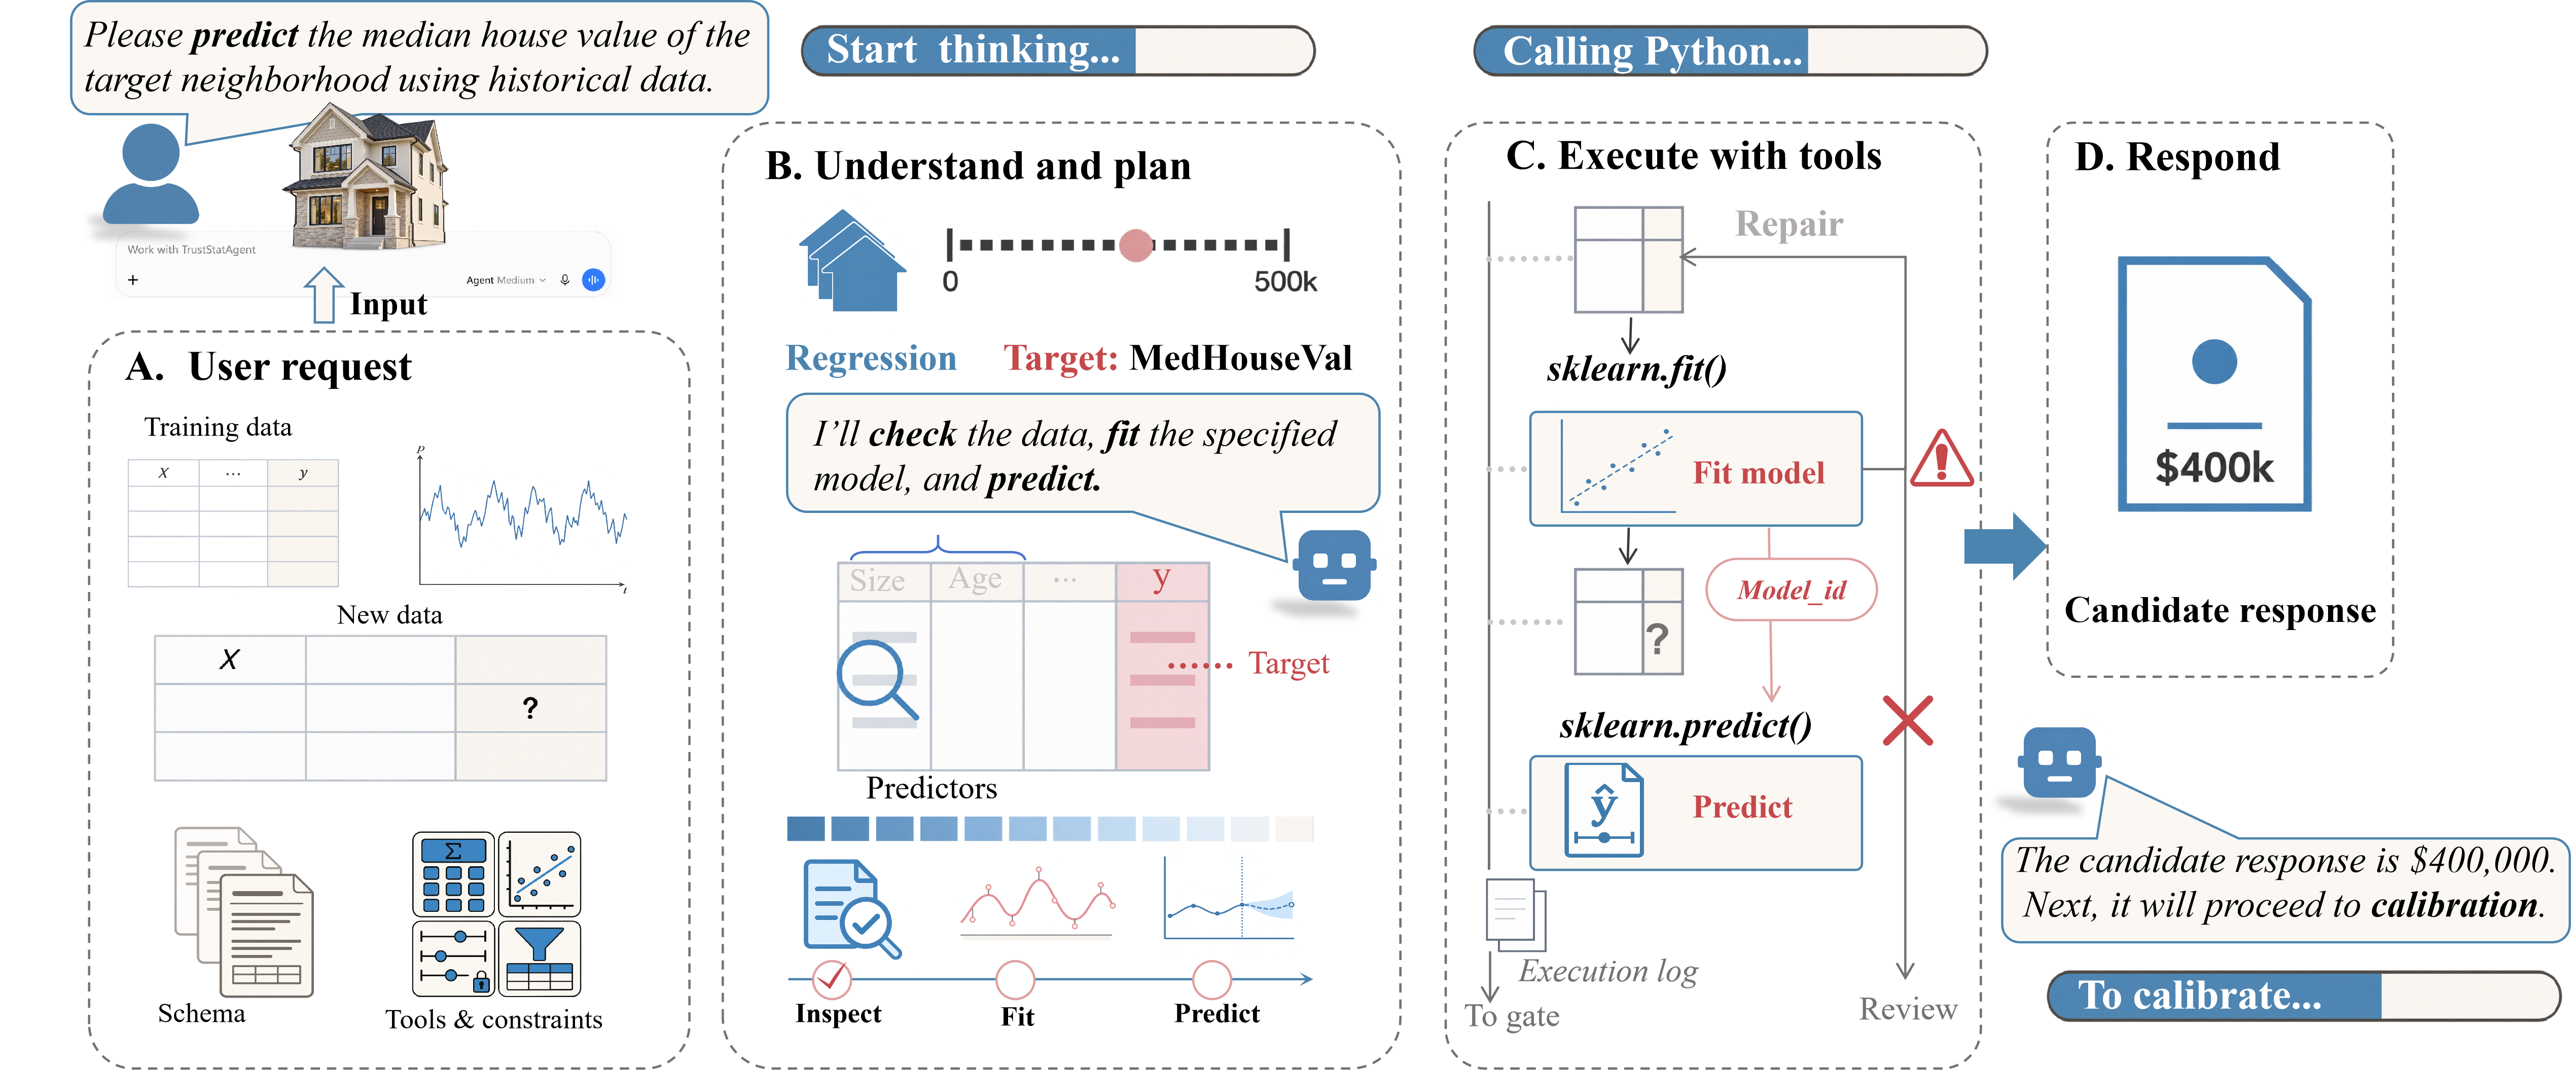
\includegraphics[width=\linewidth]{figures/sci1.png}
    \caption{LLM task planning and statistical tool execution. \textcolor{blue}{It shows how a natural-language request becomes a structured plan and a sequence of authorized tool calls, using a house-value prediction request as the running example.}}
    \label{fig:planning_execution}
\end{figure}

\subsection{Conformal uncertainty calibration}
\label{sec:uncertainty_calibration}
For each candidate result, the calibration module constructs an interval or prediction set for the corresponding target using scores computed on calibration data. Following the
conformal prediction framework \citep{angelopoulos2023gentle}, the target
is the response value for regression and forecasting, the class label
for classification, and candidate correctness for statistical question
answering. The resulting intervals and prediction sets are evaluated against the release criteria defined in Section 3.4 to determine whether each candidate result can be released automatically.

Let \(R_i\) denote the candidate generated from observable inputs \(x_i\),
and let \(T_i\) denote its calibration target. A nonconformity score
\(s_\tau(x_i,R_i,T_i)\) measures their incompatibility for task type
\(\tau\), with larger values indicating greater incompatibility.
Predictors, preprocessing procedures, and correctness scorers are fitted
separately from the records used to calculate calibration scores.

For \(n\) calibration scores ordered as
\(s_{(1)}\leq\cdots\leq s_{(n)}\), the operational threshold at nominal
miscoverage level \(\alpha\) is
\begin{equation}
    k_\alpha
    =
    \left\lceil(n+1)(1-\alpha)\right\rceil,
    \qquad
    \widehat q_\alpha
    =
    s_{(\min\{k_\alpha,n\})}.
    \label{eq:calibration_threshold}
\end{equation}
The corresponding calibrated set is
\begin{equation}
    C_\alpha(x_i,R_i)
    =
    \left\{
        u\in\mathcal{Y}_\tau:
        s_\tau(x_i,R_i,u)\leq\widehat q_\alpha
    \right\},
    \label{eq:calibrated_target_set}
\end{equation}
where \(\mathcal{Y}_\tau\) is the target space. Scores and thresholds are calculated separately for each
task setting.
Figure~\ref{fig:conformal_calibration} summarizes the four
task-specific calibration procedures described below.

\begin{figure}[H]
    \centering
    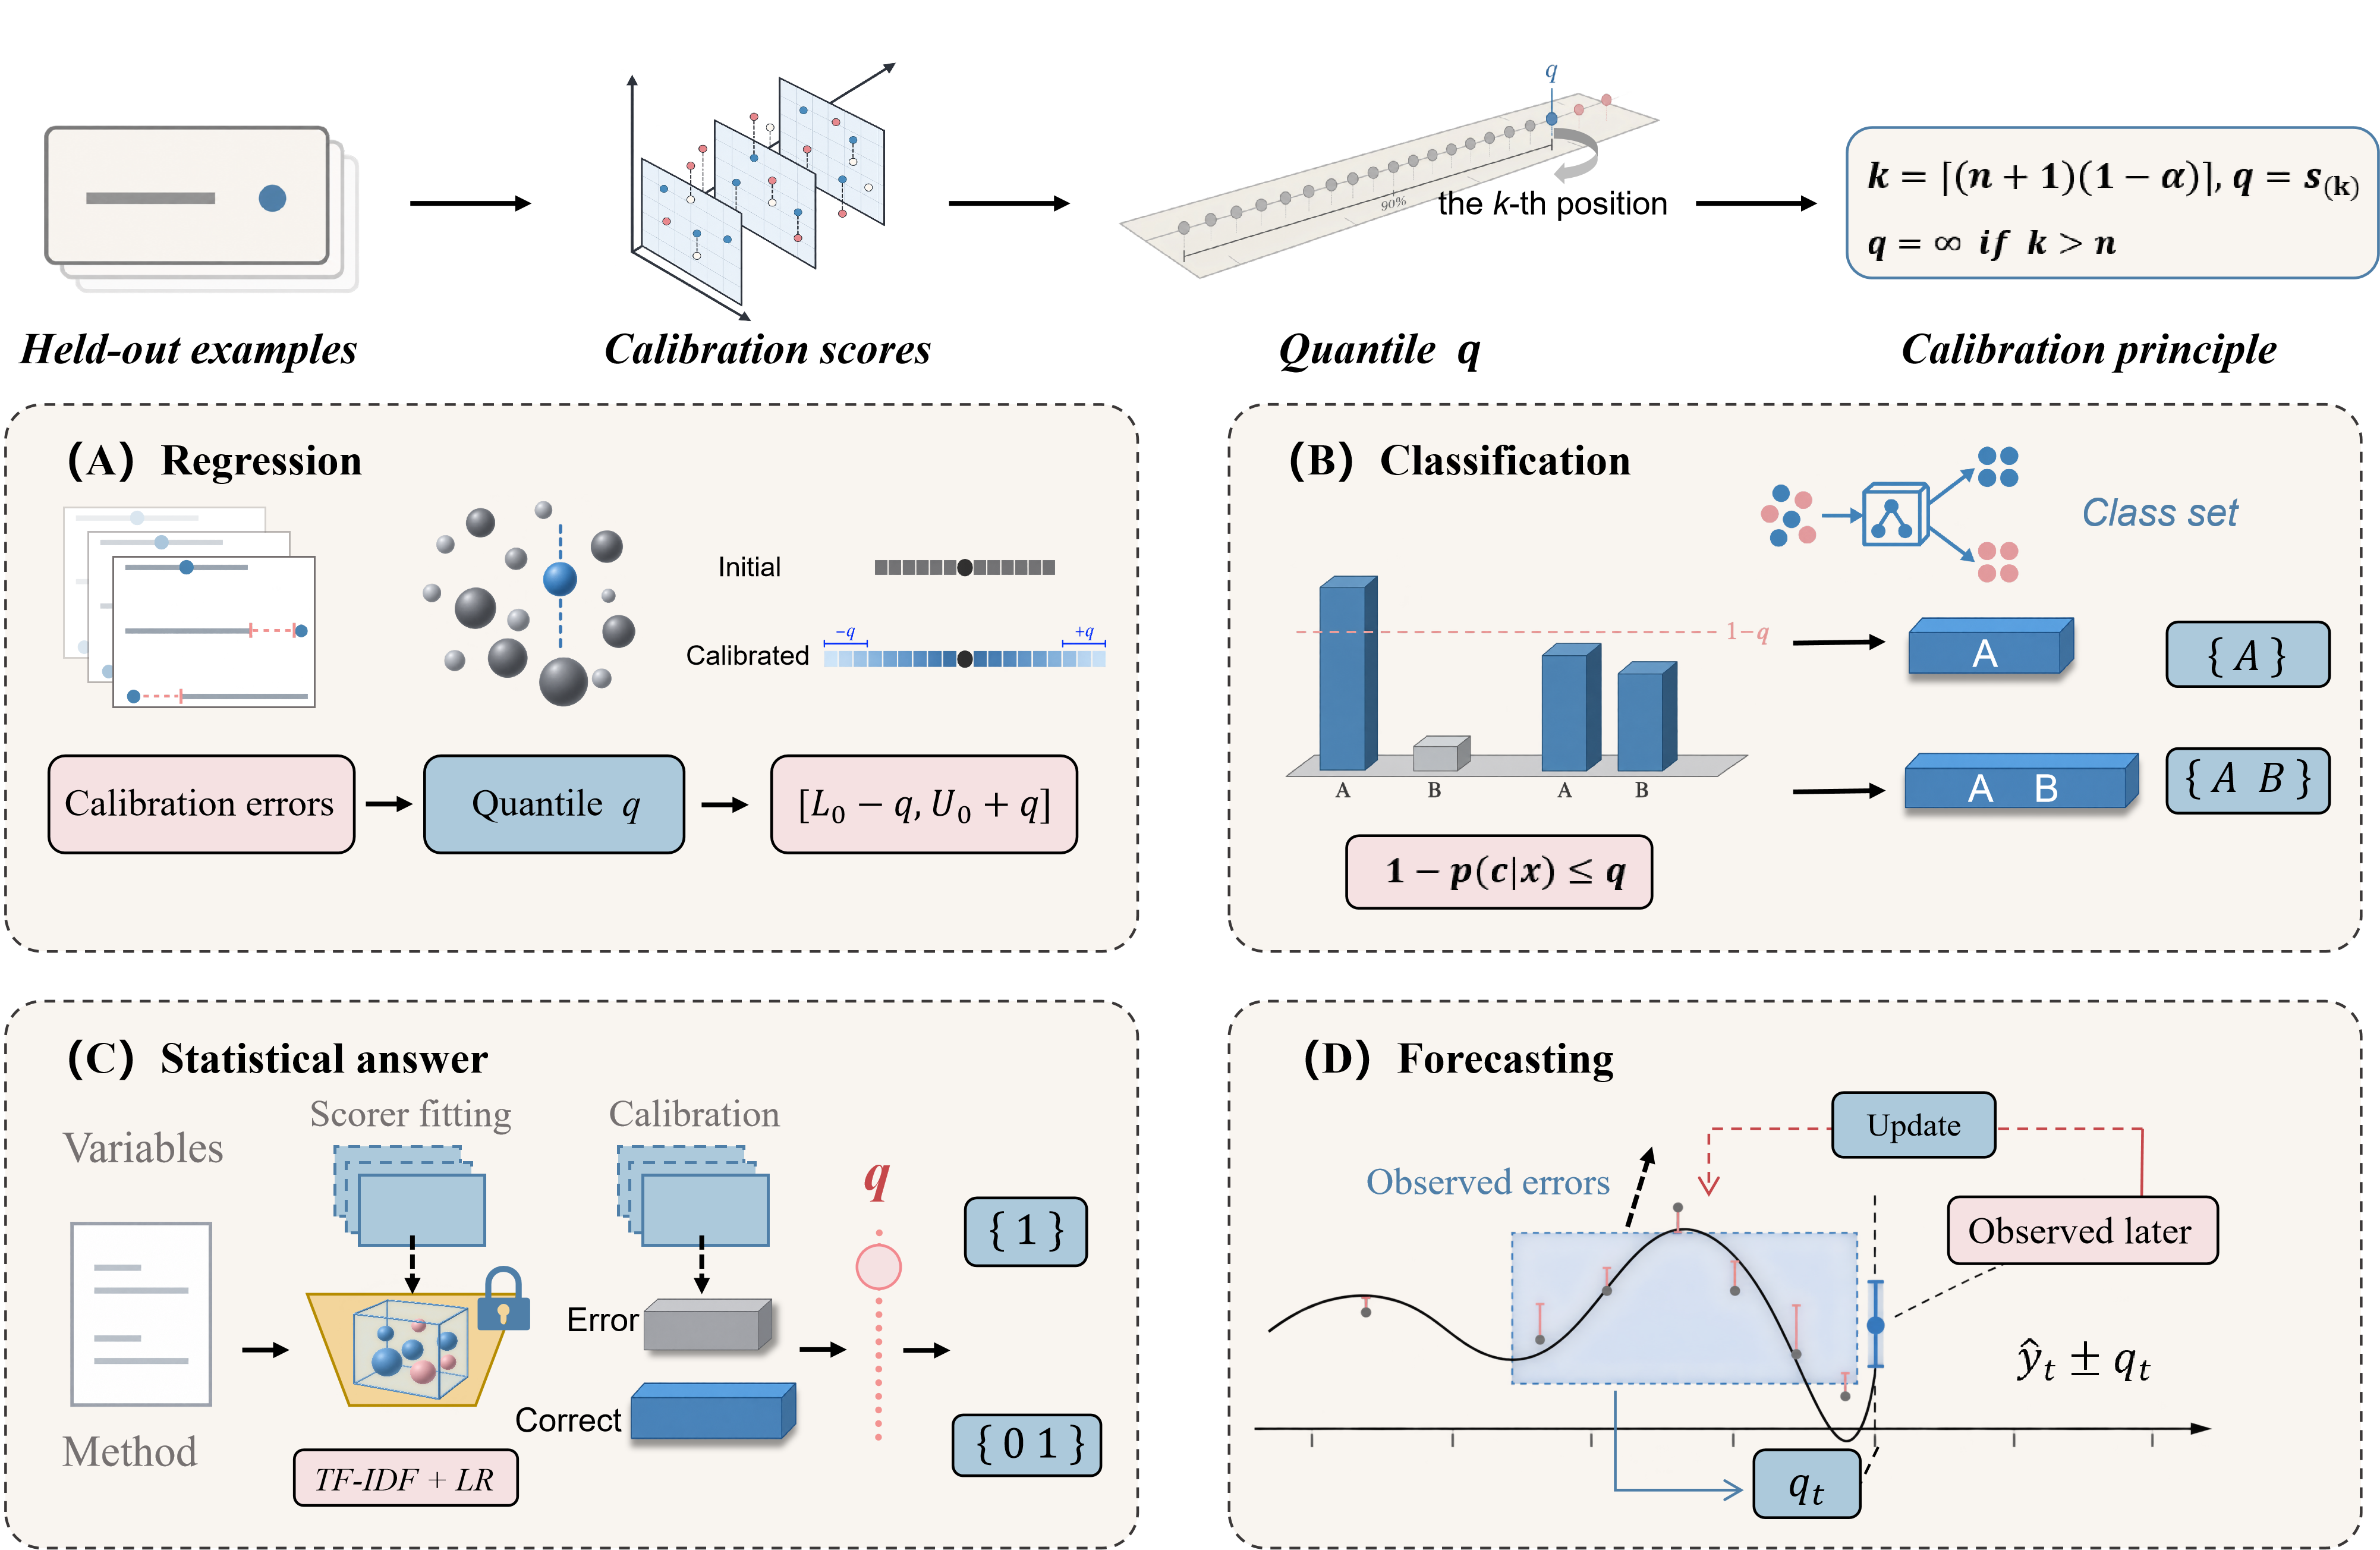
\includegraphics[width=\linewidth]{figures/sci2.png}
    \caption{Task-specific conformal uncertainty calibration. \textcolor{blue}{It depicts the four task-specific procedures that turn held-out nonconformity scores into intervals or prediction sets.}}
    \label{fig:conformal_calibration}
\end{figure}

\begin{itemize}

    \item \textbf{Numerical prediction.}
    For California Housing, we use conformalized quantile regression
    \citep{romano2019cqr}. Given preliminary lower and upper quantile
    estimates \(L_0(x)\) and \(U_0(x)\), the calibration score is
    \begin{equation}
        s_i
        =
        \max\left\{
            L_0(x_i)-y_i,\;
            y_i-U_0(x_i)
        \right\}.
        \label{eq:cqr_nonconformity}
    \end{equation}
    With \(q^{+}=\max\{0,\widehat q_\alpha\}\), the calibrated interval is
    \begin{equation}
        C_i
        =
        \left[
            L_0(x_i)-q^{+},\;
            U_0(x_i)+q^{+}
        \right].
        \label{eq:cqr_calibrated_interval}
    \end{equation}
    The adjustment preserves variation in the preliminary interval
    widths across inputs, while the nonnegative correction prevents
    calibration from contracting the interval. The point prediction
    is retained separately for the subsequent tolerance-based
    release test.

    \item \textbf{Categorical prediction.}
    For {\color{blue}Covertype}, the fitted classifier supplies class probabilities
    \(p(c\mid x_i)\). We use probability-threshold calibration
    \citep{angelopoulos2023gentle}, with scores
    \(s_i=1-p(y_i\mid x_i)\) and prediction sets
    \begin{equation}
        C_i
        =
        \left\{
            c:
            1-p(c\mid x_i)\leq\widehat q_\alpha
        \right\}.
        \label{eq:categorical_prediction_set}
    \end{equation}
    The resulting set may be empty, contain a single class, or retain
    multiple competing classes. It is passed to the gate together
    with the original predicted class, allowing release decisions
    to account for classification ambiguity.

    \item \textbf{Structured statistical answers.}
    Selective assessment requires an explicit criterion for output
    correctness \citep{lee2024selective}. For StatQA, let \(Z_i=1\)
    when the candidate's selected variables and statistical methods
    both match the reference sets under the benchmark's normalized
    exact-match criterion, and \(Z_i=0\) otherwise.

    A correctness scorer, trained on a separate scorer-training split
    and then frozen, produces \(r_i\in[0,1]\) from the observable task
    category and the generated selections. Calibration uses
    \begin{equation}
        s_i
        =
        Z_i(1-r_i)+(1-Z_i)r_i,
        \label{eq:statqa_nonconformity}
    \end{equation}
    yielding the correctness set
    \begin{equation}
        C_i
        =
        \left\{
            z\in\{0,1\}:
            z(1-r_i)+(1-z)r_i\leq\widehat q_\alpha
        \right\}.
        \label{eq:statqa_correctness_set}
    \end{equation}
    Reference answers supply offline training and calibration labels
    but are excluded from the scorer's inputs when assessing a new
    candidate. Thus, the calibrated target concerns the benchmark's
    structured analytical choices rather than unrestricted
    natural-language factuality.

    \item \textbf{Temporal prediction.}
    Online conformal methods explicitly address sequential calibration
    \citep{angelopoulos2024online}. For {\color{blue}Power Price}, we use a
    chronological rolling-residual construction around the {\color{blue}day-ahead forecast selected by the task protocol}. At time \(t\), let
    \(\mathcal{W}_t\) index the most recent \(w\) forecasts whose
    outcomes have already been observed. Their scores are
    \begin{equation}
        s_j
        =
        \left|y_j-\widehat y_j\right|,
        \qquad j\in\mathcal{W}_t.
        \label{eq:rolling_residual_scores}
    \end{equation}
    Applying Eq.~\eqref{eq:calibration_threshold} to these scores
    gives \(q_{\alpha,t}\) and the interval
    \begin{equation}
        C_t
        =
        \left[
            \widehat y_t-q_{\alpha,t},\;
            \widehat y_t+q_{\alpha,t}
        \right].
        \label{eq:rolling_calibrated_interval}
    \end{equation}
    {\color{blue}Because day-ahead prices settle with a delay, the window \(\mathcal{W}_t\) contains only forecasts whose outcomes were observed at least 24 hours before the forecast origin, so every score enters calibration after its outcome is known and never before.}

\end{itemize}



\subsection{Risk gating and selective release}
\label{sec:risk_gating}

The risk gate converts calibrated uncertainty into a decision about
automatic release. Recent work on informative conformal prediction examines how
prediction sets can be selected to meet application needs
\cite{gazin2025selecting}, while conformal risk control uses
specified loss functions to calibrate prediction rules
\cite{angelopoulos2024conformal}. In our framework, the
release criteria define which target values are acceptable.
A candidate is eligible for automatic release only if every
value or label in its calibrated set meets these criteria.

Let \(\mathcal{A}_{\Omega,i}\) denote the acceptable target set for
candidate \(i\), with requirements \(\Omega\) fixed before test
evaluation. Let \(H_i=1\) indicate an unresolved execution failure,
and let \(V_i=1\) indicate an available, valid uncertainty output.
Numerical intervals must have finite, ordered endpoints, while
discrete sets must be nonempty and contain admissible labels.
The release decision is
\begin{equation}
    g_i
    =
    \mathbf{1}\{H_i=0\}
    \mathbf{1}\{V_i=1\}
    \mathbf{1}\{C_i\subseteq\mathcal{A}_{\Omega,i}\},
    \label{eq:unified_release_gate}
\end{equation}
where \(g_i=1\) denotes automatic release and \(g_i=0\) denotes referral.
The validity condition excludes empty sets, whose mathematical
containment in any acceptance set would otherwise permit release
without supporting evidence.

For numerical predictions, the acceptable target set is
\begin{equation}
    \mathcal{A}_{\Omega,i}
    =
    \left[
        \widehat y_i-\Delta,\;
        \widehat y_i+\Delta
    \right],
    \label{eq:numerical_acceptance_set}
\end{equation}
where \(\Delta>0\) specifies the permitted prediction error.
Containment checks both interval endpoints relative to the point
prediction. For categorical
predictions, the acceptable set is the predicted-class singleton;
for StatQA, it is the correctness label \(\{1\}\).
Table~\ref{tab:calibrated_release_conditions} summarizes the
resulting conditions.
\textcolor{red}{For StatQA the release test thresholds the calibrated correctness score, \(g_i=1\) when \(r_i\geq\tau\); \(\tau\) is fixed on the validation split under the same pre-registered release-band rule as the other benchmarks, targeting roughly 60\% automatic release, and the prediction set \(C_i\) still accompanies every candidate as its coverage certificate.}

\begin{table}[t]
    \centering
    \caption{Automatic-release conditions. All conditions additionally
    require successful execution and a valid uncertainty output.}
    \label{tab:calibrated_release_conditions}
    \small
    \renewcommand{\arraystretch}{1.2}
    \begin{tabular}{@{}lll@{}}
        \toprule
        \textbf{Output type}
        & \textbf{Calibrated output}
        & \textbf{Release condition} \\
        \midrule

        Regression
        & \([L_i,U_i]\)
        & \(L_i\geq\widehat y_i-\Delta\), \(U_i\leq\widehat y_i+\Delta\) \\

        Classification
        & Class set \(C_i\)
        & \textcolor{red}{\(\widehat p(\widehat y_i\mid x_i)\geq\tau\), \(\tau\) fixed on validation} \\

        Statistical QA
        & Correctness set \(C_i\)
        & \textcolor{red}{\(r_i\geq\tau\), \(\tau\) fixed on validation} \\

        Forecasting
        & \(\widehat y_t\pm q_{\alpha,t}\)
        & \(q_{\alpha,t}\leq\Delta\) \\

        \bottomrule
    \end{tabular}
\end{table}

The gate automatically releases a candidate when execution
succeeds, the uncertainty output is valid, and the acceptance
criterion is satisfied. All remaining candidates are referred
for review.
Figure~\ref{fig:risk_gating} illustrates the checks,
acceptance tests, and routing decisions of the risk gate.

\begin{figure}[H]
    \centering
    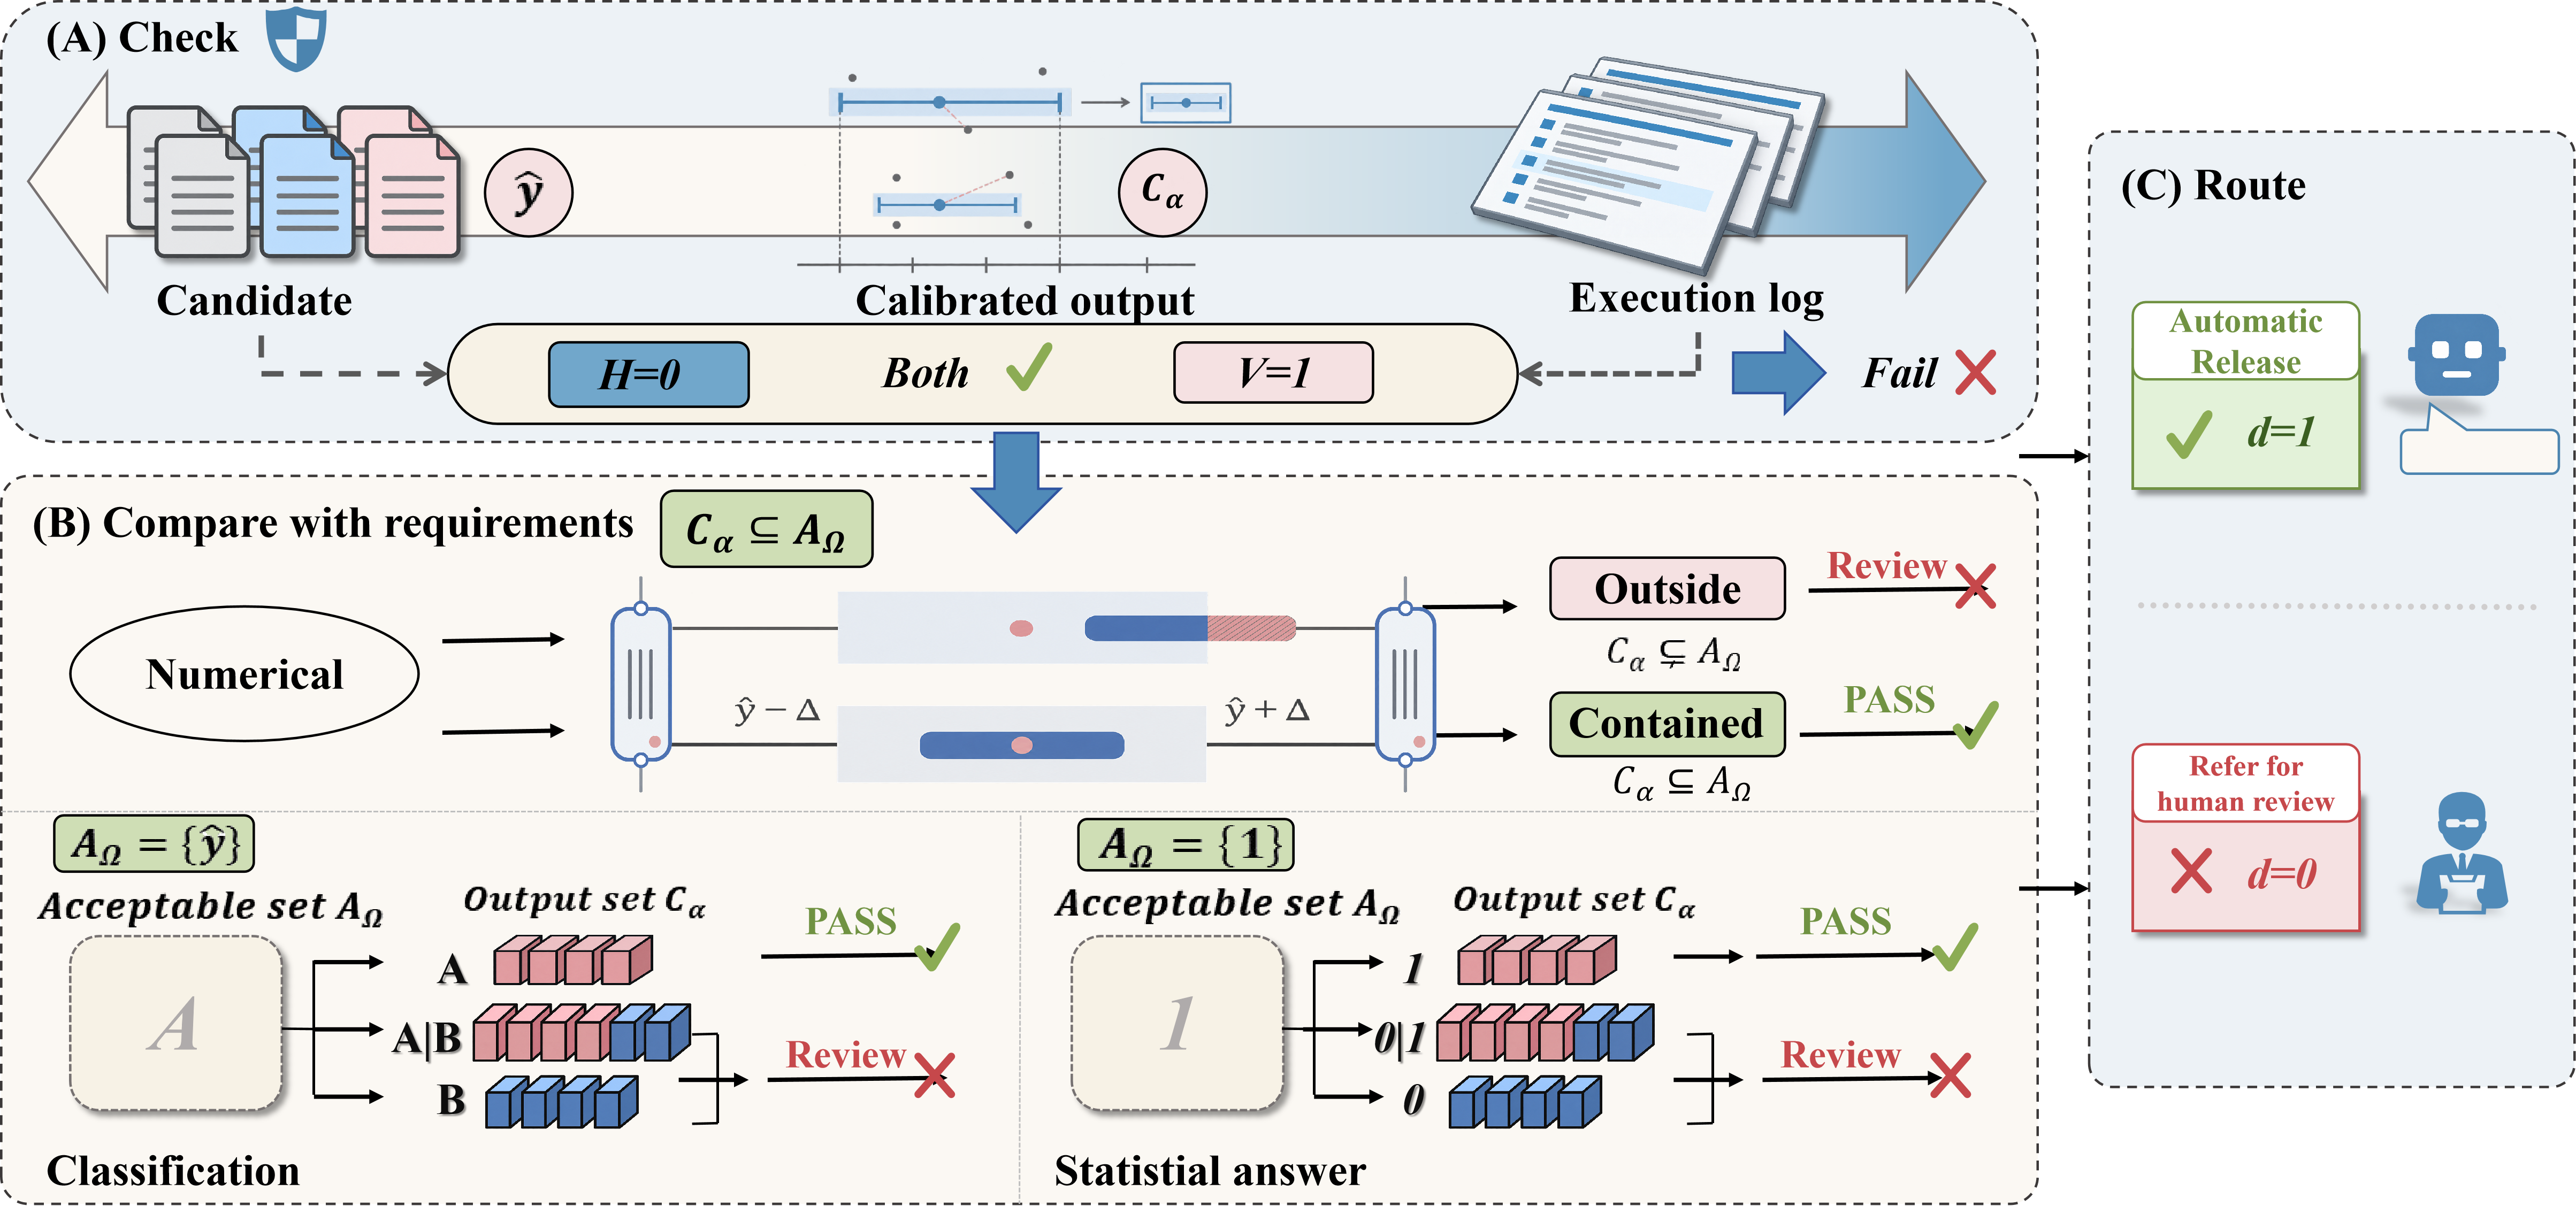
\includegraphics[width=\linewidth]{figures/sci3.png}
    \caption{Risk gating and selective release. \textcolor{blue}{It depicts the checks, acceptance tests, and routing decisions that turn a calibrated output into a release or a referral.}}
    \label{fig:risk_gating}
\end{figure}
\textcolor{red}{For the interval- and set-valued outputs, the} containment rule also clarifies the connection between calibration
and release. If \(g_i=1\), then
\(C_i\subseteq\mathcal{A}_{\Omega,i}\); therefore,
\begin{equation}
    \left\{
        g_i=1,\;
        T_i\notin\mathcal{A}_{\Omega,i}
    \right\}
    \subseteq
    \left\{
        T_i\notin C_i
    \right\}.
    \label{eq:release_violation_inclusion}
\end{equation}
Thus, whenever a released result violates the acceptance
criterion, the true target lies outside the calibrated set.
A valid upper bound on marginal miscoverage therefore also
bounds the probability of a release error. The error rate
among released results requires separate evaluation because
it is calculated within the subset selected by the gate
\citep{jin2025confidence}. We therefore report empirical
coverage, release rate, and error rate among released
candidates together.


\section{Experimental Setup}
\label{sec:experimental_setup}

\subsection{Benchmark tasks and datasets}
\label{sec:benchmark_tasks}

{\color{blue}
Four benchmarks cover the four output types a statistical agent produces in practice, namely a structured analytical answer, a class label, a point prediction, and a day-ahead price forecast.
Table~\ref{tab:benchmark_tasks} summarises their roles.
The acceptance rule in the last column defines what counts as an error for the release decision, and everything the gate lets through must satisfy it.
}

\begin{table}[H]
    \centering
    \caption{\textcolor{blue}{Benchmark tasks. The acceptance rule defines an error for the release decision; $\Delta$ is a validation-selected tolerance in the dataset's target unit.}}
    \label{tab:benchmark_tasks}
    \small\color{blue}
    \setlength{\tabcolsep}{4pt}
    \renewcommand{\arraystretch}{1.2}
    \begin{tabularx}{\linewidth}{
        @{}
        l
        >{\raggedright\arraybackslash}p{0.15\linewidth}
        >{\raggedright\arraybackslash}X
        >{\raggedright\arraybackslash}p{0.20\linewidth}
        >{\raggedright\arraybackslash}p{0.16\linewidth}
        @{}
    }
        \toprule
        \textbf{Benchmark}
        & \textbf{Task}
        & \textbf{Candidate output}
        & \textbf{Calibrated output}
        & \textbf{Acceptance rule} \\
        \midrule
        StatQA
        & Statistical analysis QA
        & Variable and method selection with the computed answer
        & Calibrated correctness score
        & Official correctness criterion \\

        Covertype
        & 7-class classification
        & Predicted class with class probabilities
        & Conformal prediction set
        & Correct predicted class \\

        California Housing
        & Regression
        & Point prediction with quantile interval
        & Conformalized prediction interval
        & $|y-\hat{y}|\le\Delta$ \\

        Power Price
        & Day-ahead forecasting
        & 24\,h-ahead price forecast with quantile interval
        & Rolling conformal interval
        & $|y-\hat{y}|\le\Delta$ \\
        \bottomrule
    \end{tabularx}
\end{table}

\begin{enumerate}
    \renewcommand{\labelenumi}{\color{blue}\arabic{enumi}.}
    \setlength{\itemsep}{6pt}
    \color{blue}

    \item \textbf{StatQA.}
    StatQA~\citep{zhu2024large} evaluates the selection of relevant variables and applicable statistical methods.
    All experiments use mini-StatQA, the stratified subset of 1{,}163 examples released with the benchmark, which preserves the task-category and difficulty distribution of the full collection.
    The benchmark authors conduct all of their own evaluation on this subset~\citep{zhu2024large}, so our results are directly comparable to the published reference numbers.
    The 1{,}163 items are divided per task category into scorer-calibration, conformal-calibration, validation, and test splits in the ratio 20/20/20/40; the scorer-calibration split trains the answer-correctness scorer.

    \item \textbf{Covertype.}
    Covertype~\citep{blackard1999comparative} assigns 581{,}012 instances described by 54 cartographic variables to one of seven forest cover types, with pronounced class imbalance.
    We evaluate on a stratified random sample of 100{,}000 instances, of which 50{,}000 train the classifier and the calibration, validation, and test partitions contain 15{,}000, 15{,}000, and 20{,}000 instances.

    \item \textbf{California Housing.}
    California Housing~\citep{pace1997sparse} requires predicting the median house value of 20{,}640 districts.
    The calibration, validation, and test partitions contain 3{,}096, 3{,}096, and 4{,}128 instances.

    \item \textbf{Power Price.}
    The forecasting benchmark uses hourly day-ahead auction prices of the Germany--Luxembourg bidding zone published by Energy-Charts~\citep{energycharts2025}, covering 2023--2025.
    At day $d$ the agent forecasts each hourly price of day $d{+}1$.
    The protocol is strictly causal. Features are restricted to information available at the forecast origin, the forecaster is selected from a fixed model pool by chronological cross-validation with a 24-hour embargo, and rolling conformal calibration observes a 24-hour feedback delay.
    Ridge regression with $\alpha=10$ is selected on all three seeds.
    The calibration, validation, and test partitions contain 3{,}892, 3{,}892, and 5{,}200 hourly targets.

\end{enumerate}

\subsection{Evaluation protocol}
\label{sec:evaluation_protocol}

{\color{blue}
The comparison is organised around one principle. Every release rule evaluated below consumes the same candidate pool, generated once per benchmark and stored, so methods differ only in how they decide what to publish.

All experiments use three seeds. On StatQA, whose candidates are frozen language-model outputs, a seed reshuffles how the items are assigned to the four splits; on the predictive benchmarks a seed also varies model initialisation, and the pipelines are refit under each seed.
All thresholds are selected on the validation split, all conformal quantities on the calibration split, and the test partition is evaluated once, after every operating point has been fixed.

A released result is an error when it violates the acceptance rule of its task (Table~\ref{tab:benchmark_tasks}).
Write $g_i = 1$ when candidate $i$ is released automatically and $v_i = 1$ when it violates the acceptance rule.
Two quantities summarise every release policy.
The release rate measures the fraction of candidates published automatically,
\begin{equation}
    \text{Release rate}
    =
    \frac{1}{N}\sum_{i=1}^{N} g_i,
    \label{eq:exp_release_rate}
\end{equation}
and the released error rate measures the fraction of published candidates that violate the acceptance rule,
\begin{equation}
    \text{Released error rate}
    =
    \frac{\sum_{i=1}^{N} g_i\, v_i}
         {\sum_{i=1}^{N} g_i}.
    \label{eq:exp_released_error_rate}
\end{equation}
A reliability figure never appears without the release rate at which it was attained, since any error rate can be driven to zero by releasing nothing.

Gating studies are frequently compared at each method's own operating point, which conflates the quality of the risk ranking with the choice of threshold.
We therefore evaluate every rule under a \emph{matched-release} protocol. At each target rate $r\in\{20,40,60,80\}\%$, each rule releases exactly the $r$ fraction of the test partition it ranks as least risky, with ties broken by a pre-fixed sample index, and released error rates are compared at an identical level of automation.
Significance is assessed by a paired bootstrap~\citep{efron1993introduction} on the per-sample difference of released errors against TrustStatAgent with 1{,}000 replicates; because the hourly price series is autocorrelated, Power Price uses a circular block bootstrap~\citep{politis1992circular} with a block length of 168 hours.
A difference is called significant when its 95\% confidence interval excludes zero.

Finally, sweeping the release rate from 5\% to 100\% traces a risk--coverage curve~\citep{elyaniv2010foundations} per method, and the area under this curve (AURC)~\citep{geifman2017selective} summarises the whole spectrum in one number, reported in units of $10^{-2}$.
AURC protects the comparison against single-point tuning, since a method that is ahead only at a carefully chosen operating point does not attain a low AURC.
The quality of the calibrated output itself is measured by empirical coverage against its nominal level~\citep{angelopoulos2023gentle},
\begin{equation}
    \widehat{\mathrm{Coverage}}
    =
    \frac{1}{|I_{\mathrm{cov}}|}
    \sum_{i\in I_{\mathrm{cov}}}
    \mathbf{1}\{y_i\in C_i\},
    \label{eq:exp_coverage}
\end{equation}
computed over all test candidates with observed targets before any release decision is taken.
}

\subsection{Comparative methods}
\label{sec:comparative_methods}

{\color{blue}
Eight reference methods stand against the release layer of TrustStatAgent. Selective-prediction methods rank candidates by a confidence score and reject the tail, conformal methods add distribution-free guarantees to a ranking, and end-to-end references carry no per-sample reliability signal and cannot be gated at all.
Table~\ref{tab:comparative_methods} lists them with the release rule each one applies and its key difference from the proposed gate.
All of them operate on the frozen candidate pools of Section~\ref{sec:evaluation_protocol}; the end-to-end references produce their own candidates, publish every one of them, and mark what a pipeline without a release layer looks like.
}

\begin{table}[t]
    \centering
    \caption{\textcolor{blue}{Comparative methods. All gating methods consume the identical frozen candidates; only the release rule differs.}}
    \label{tab:comparative_methods}
    \scriptsize\color{blue}
    \setlength{\tabcolsep}{3pt}
    \renewcommand{\arraystretch}{1.15}
    \begin{tabularx}{\linewidth}{
        @{}
        >{\raggedright\arraybackslash}p{0.12\linewidth}
        >{\raggedright\arraybackslash}p{0.19\linewidth}
        >{\raggedright\arraybackslash}X
        >{\raggedright\arraybackslash}p{0.22\linewidth}
        @{}
    }
        \toprule
        \textbf{Family}
        & \textbf{Method}
        & \textbf{Release rule}
        & \textbf{Key difference from ours} \\
        \midrule

        ---
        & TrustStatAgent (ours)
        & Fused calibrated risk (interval width, error model, rolling residuals, answer agreement) + execution checks; deterministic risk gate
        & --- \\

        \midrule
        \multirow{6}{*}{\shortstack[l]{Selective\\prediction}}

        & Selective threshold \citep{chow1970optimum,geifman2017selective}
        & Threshold on $1-\max_c \hat{p}_c$ or interval half-width
        & Single hand-crafted signal \\

        & Learned error model \citep{geifman2019selectivenet}
        & Threshold on a trained error-probability scorer
        & Single learned signal; no coverage certificate \\

        & Verbalized confidence \citep{kadavath2022language}
        & Threshold on self-reported probability of correctness
        & Uncalibrated self-report only \\

        \midrule
        \multirow{7}{*}{\shortstack[l]{Conformal\\methods}}

        & Conformal abstention \citep{vovk2005algorithmic}
        & Release only when the prediction set is a singleton
        & Binary signal; often inoperative \\

        & CRC (LTT) \citep{angelopoulos2024conformal}
        & Learn-then-test threshold with distribution-free risk control
        & Same single signal as selective thresholding; guarantee only fixes the threshold \\

        & ACI \citep{gibbs2021adaptive}
        & Threshold on online-updated interval width
        & Time-series only; single signal \\

        \midrule
        \multirow{4}{*}{\shortstack[l]{End-to-end\\reference}}

        & Zero-shot-CoT \citep{kojima2022large}
        & No reliability signal; publishes all
        & Cannot be gated \\

        & ReAct direct \citep{yao2023react}
        & Interleaved tool use without calibration or a gate
        & Cannot be gated \\

        \bottomrule
    \end{tabularx}
\end{table}

{\color{blue}
Two relations among the baselines deserve note.
CRC ranks candidates by the same score as selective thresholding; the two differ in how the operating point is chosen, validation tuning against risk control, so their matched-release rows coincide in Section~\ref{sec:results_matched} and any gap between them in the tables reflects threshold selection alone.
The verbalized-confidence baseline presupposes a generated answer to self-assess and is therefore evaluated on StatQA, the benchmark whose candidates are produced by the language model; ACI is evaluated on Power Price, the benchmark with a temporal structure.
The learned error model does not appear on StatQA because the calibrated correctness scorer of Section~\ref{sec:execution} is itself a learned error score, so the two rows would coincide by construction.
}

\subsection{Ablation studies}
\label{sec:ablation_studies}

{\color{blue}
Three ablations examine the contribution of each module of the release layer.
Each variant removes one component while retaining every other setting, and thresholds are not retuned to compensate for the removal, so any performance change is attributable to the removed component alone.
}

{\color{blue}
\textbf{Without explicit planning.}
The agent omits the structured plan but retains the same task inputs, tools, and execution budget; evaluated on StatQA under the official correctness criterion, this variant measures what the plan contributes to candidate quality.

\textbf{Without conformal calibration.}
The gate keeps its fusion function and validation-selected threshold, but the calibrated interval or set signal is replaced by its uncalibrated counterpart.
This variant measures what calibration contributes to the operating point and to the coverage certificate.

\textbf{Without the risk gate.}
Calibration is retained but every candidate with a valid calibrated output is released, so the released error rate reproduces the candidate error rate and measures what the gate filters out.
}

\subsection{Language model configuration and computational budget}
\label{sec:llm_configuration}

{\color{blue}
All language-model calls in the main experiments use GPT-6.1-sol through an OpenAI-compatible API with deterministic decoding (temperature 0.0) and a completion budget of 1{,}200 tokens; every prompt is reproduced in \ref{app:prompts} and the per-benchmark call counts in \ref{app:budget}.
The release layer itself makes no language-model calls. Calibration is a property of the procedure and the gate is a deterministic program over execution records and calibrated outputs, so neither depends on the backbone that produced the candidates.
To verify that the framework transfers across backbones, Section~\ref{sec:results_multillm} repeats the main gating comparison with three further instruction-following models.
}

\section{Results}
\label{sec:results}

{\color{blue}
We first establish that the agent does real work (Section~\ref{sec:results_autonomous}), then compare release rules at a matched release rate (Section~\ref{sec:results_release}) and across the whole risk--coverage spectrum (Section~\ref{sec:results_matched}), and finally check that each module is necessary (Section~\ref{sec:results_ablation}) and that the framework transfers across language-model backbones (Section~\ref{sec:results_multillm}).
The raw counts behind every release figure are tabulated in \ref{app:counts}, and the four benchmarks are reported separately and never averaged, since their error scales differ by an order of magnitude.
}

\subsection{Autonomous planning and tool use}
\label{sec:results_autonomous}

{\color{blue}
The first question is whether the agent is doing real work or decorating a fixed pipeline.
We answer it with a four-arm study on the three predictive benchmarks, twenty tasks per benchmark.
The \emph{fixed} arm runs a reference pipeline chosen by the authors (two tool calls, no planning).
The \emph{autonomous} arm lets the agent inspect the data schema, select the statistical method, and compose the tool sequence itself.
Each arm runs with and without the risk gate, and a failure-injection probe corrupts tool outputs mid-execution to test the execution checks.
Table~\ref{tab:autonomous} reports the outcome and Figure~\ref{fig:autonomous} visualises it.
}

\begin{table}[t]
    \centering
    \caption{\textcolor{blue}{Autonomous planning study, 20 tasks per benchmark, mean over three seeds. Metric: accuracy for Covertype (higher is better), MAE for California Housing and Power Price (lower is better). Blocked: intercepted failure-injection probes; the probe aborts execution upstream of the gate, so interception is identical across arms.}}
    \label{tab:autonomous}
    \scriptsize\color{blue}
    \setlength{\tabcolsep}{2.5pt}
    \renewcommand{\arraystretch}{1.15}
    \begin{tabular}{@{}llrrrrrc@{}}
        \toprule
        \textbf{Benchmark} & \textbf{Arm}
        & \textbf{Metric} & \textbf{Release (\%)} & \textbf{Rel.\ err.\ (\%)}
        & \textbf{Plan (\%)} & \textbf{Calls} & \textbf{Blocked} \\
        \midrule
        \multirow{4}{*}{Covertype}
        & fixed                & 0.697 & 100.00 & 30.34 &   0 & 2.00 & \multirow{4}{*}{3/3} \\
        & fixed + gate         & 0.697 &  60.05 & 17.03 &   0 & 2.00 & \\
        & autonomous           & 0.887 & 100.00 & 11.27 & 100 & 4.00 & \\
        & autonomous + gate    & 0.887 &  60.02 &  1.90 & 100 & 4.00 & \\
        \midrule
        \multirow{4}{*}{Calif.\ Housing}
        & fixed                & 0.326 & 100.00 &  7.11 &   0 & 2.00 & \multirow{4}{*}{4/4} \\
        & fixed + gate         & 0.326 &  60.60 &  2.17 &   0 & 2.00 & \\
        & autonomous           & 0.319 & 100.00 &  5.44 & 100 & 4.15 & \\
        & autonomous + gate    & 0.319 &  60.35 &  1.52 & 100 & 4.15 & \\
        \midrule
        \multirow{4}{*}{Power Price}
        & fixed                & 16.70 & 100.00 &  4.47 &   0 & 2.00 & \multirow{4}{*}{3/3} \\
        & fixed + gate         & 16.70 &  59.46 &  0.87 &   0 & 2.00 & \\
        & autonomous           & 15.36 & 100.00 &  6.98 & 100 & 4.60 & \\
        & autonomous + gate    & 15.36 &  61.14 &  2.94 & 100 & 4.60 & \\
        \bottomrule
    \end{tabular}
\end{table}

\begin{figure}[H]
    \centering
    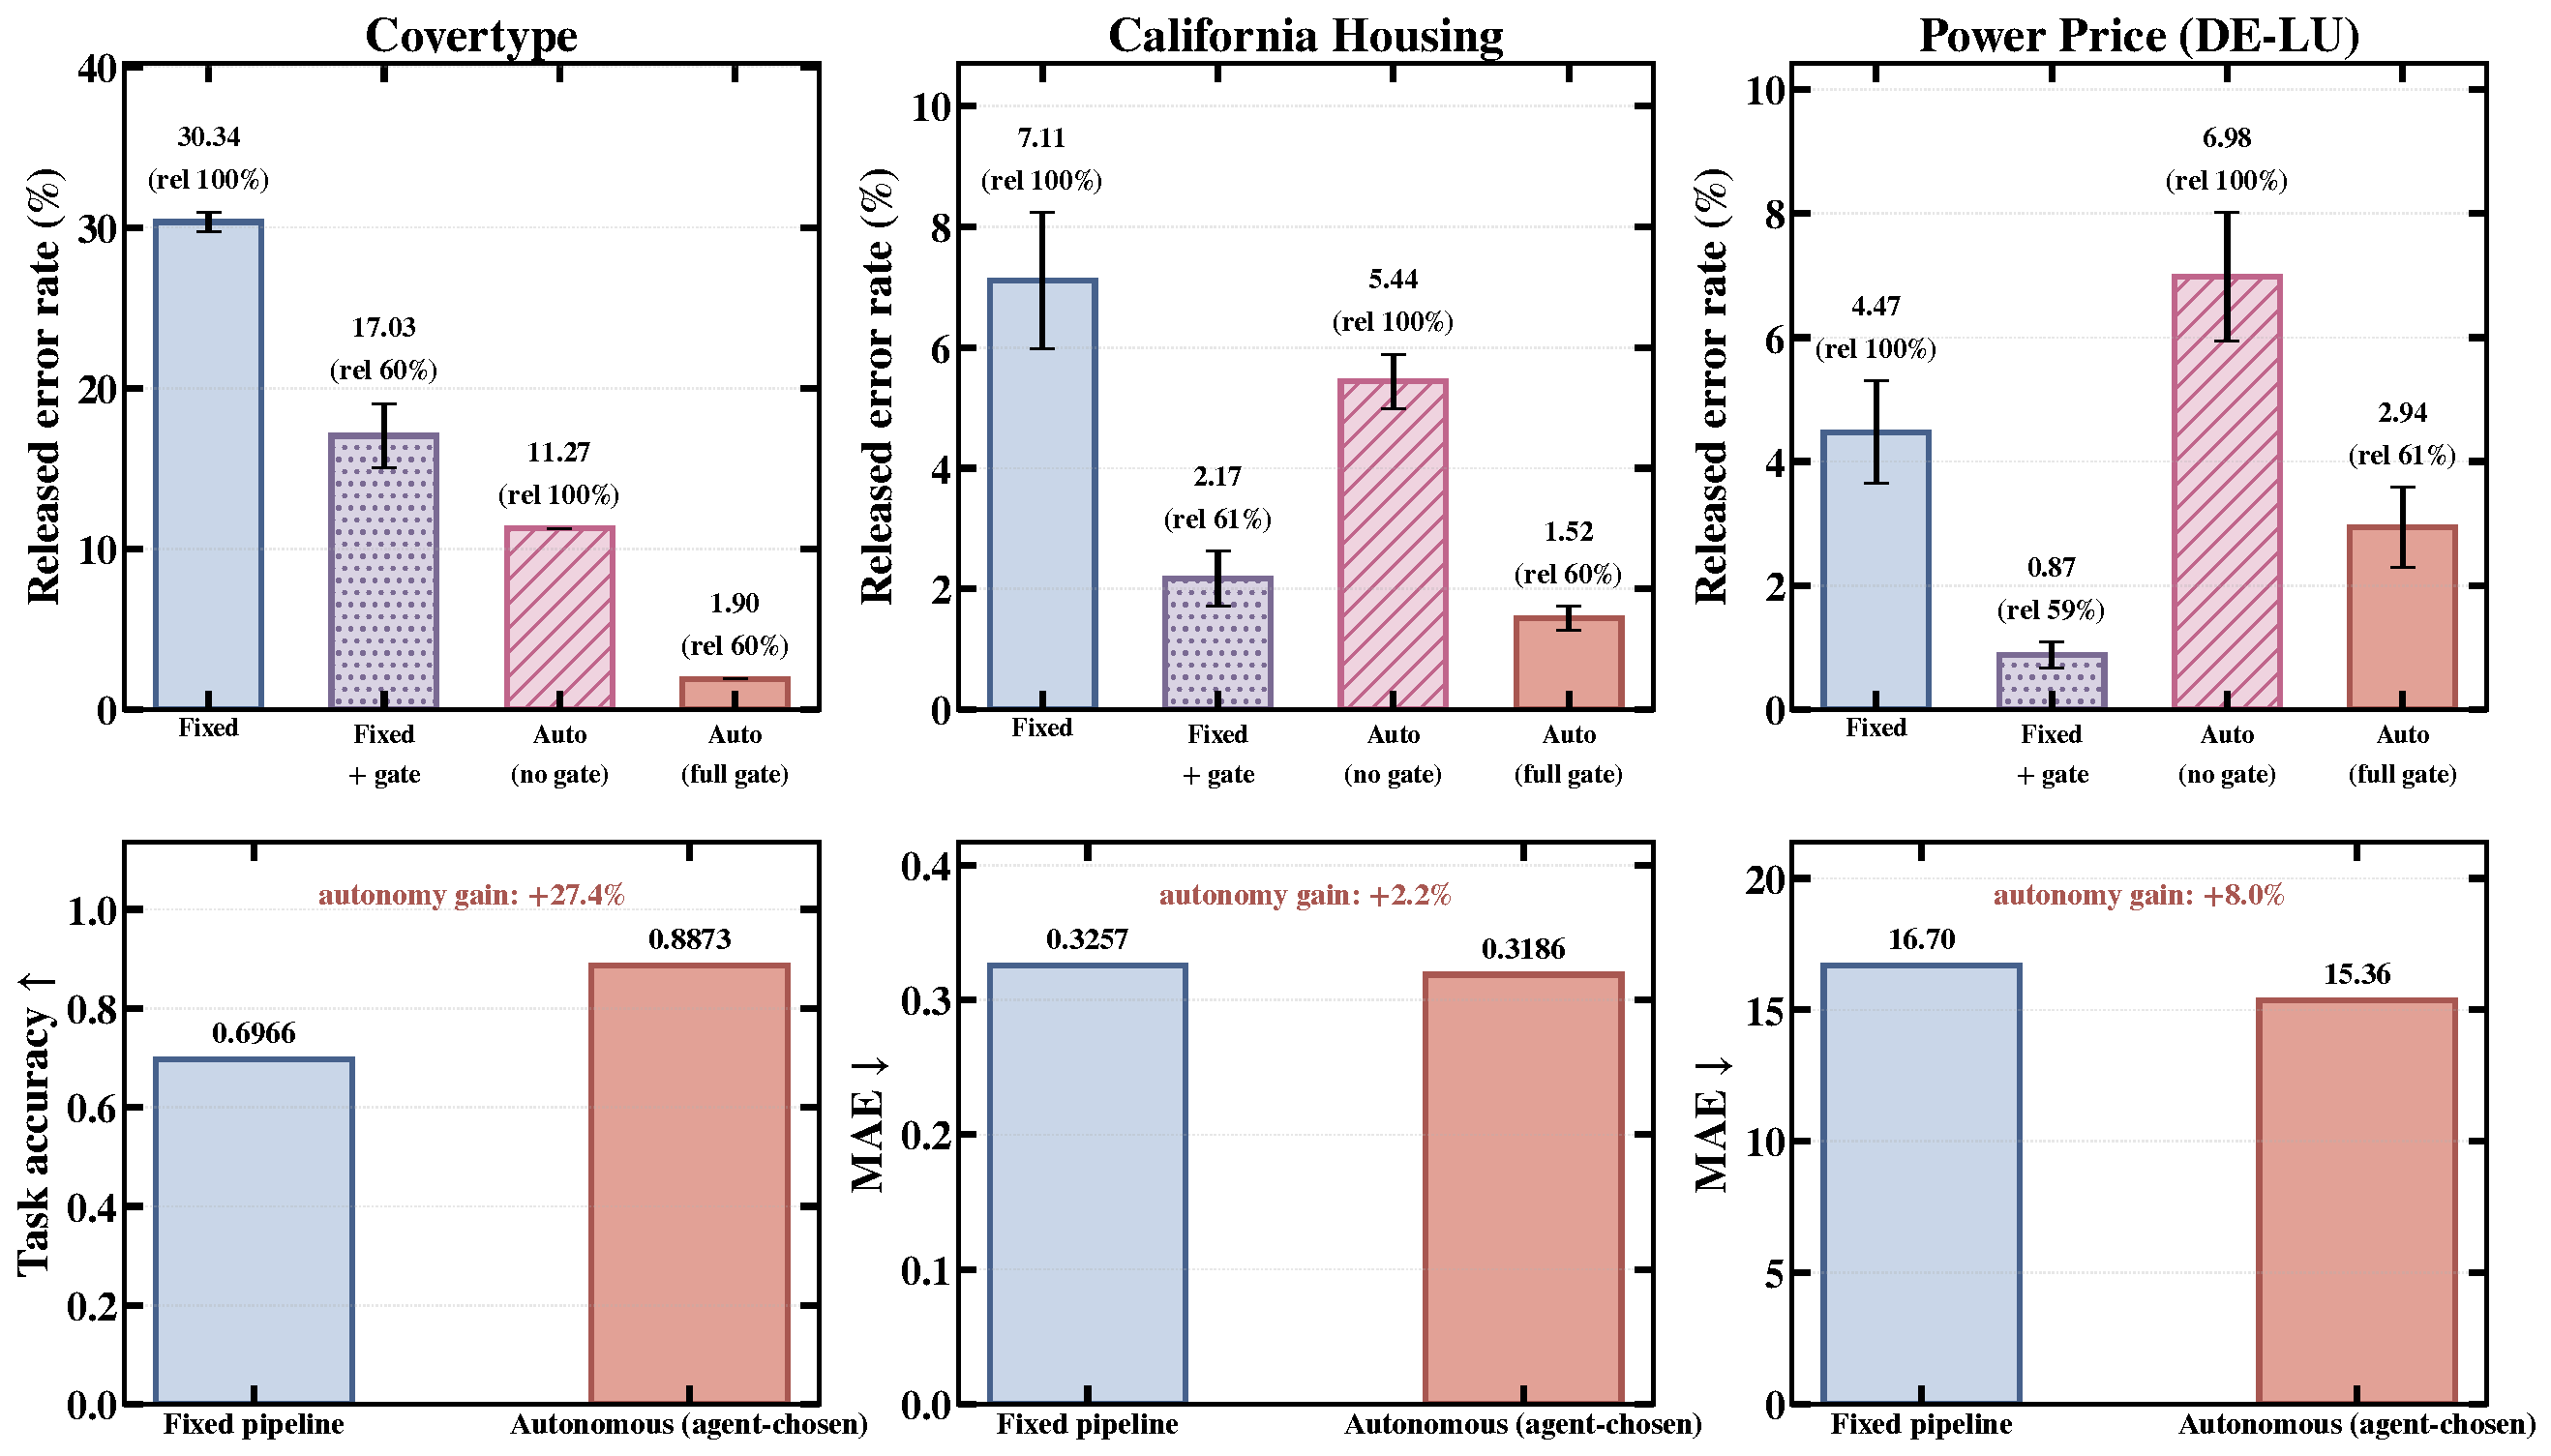
\includegraphics[width=0.95\linewidth]{figures/fig4_autonomous.pdf}
    \caption{\textcolor{blue}{Autonomous planning versus the fixed pipeline, with and without the gate.}}
    \label{fig:autonomous}
\end{figure}

{\color{blue}
The agent's plans are executable in every run and use about four tool calls against the fixed pipeline's two; that extra work is where the quality gain comes from.
On Covertype, autonomous method selection lifts accuracy from 0.697 to 0.887; on California Housing MAE improves from 0.326 to 0.319; on Power Price from 16.70 to 15.36.
On StatQA the same effect appears in the planning ablation of Section~\ref{sec:results_ablation}, where removing the plan costs 2.30 points of official accuracy.
The resulting candidate pools sit at competitive operating levels, with 56.97\% official accuracy on StatQA, 88.77\% accuracy on Covertype, MAE 0.312 on California Housing, and MAE 15.76 on Power Price.

The gate then does its own work on top of the autonomous candidates.
Comparing each autonomous arm against itself with the gate removed, the released error rate falls from 11.27\% to 1.90\% on Covertype, from 5.44\% to 1.52\% on California Housing, and from 6.98\% to 2.94\% on Power Price, reductions of 83\%, 72\%, and 58\%.
On Power Price the gated fixed arm attains a still lower released error rate of 0.87\%, and the reason is structural. The two arms gate different candidate pools, so the comparison is outside the matched-release protocol, and the fixed pipeline's violations are concentrated where any gate can see them. In the fixed pool, 85.6\% of violations fall in the highest-risk 40\% of candidates, against 62.1\% for the autonomous pool, whose smaller and more evenly spread residuals are intrinsically harder to rank.
What matters for deployment is the joint outcome, and there the autonomous gated arm pairs the best task metric, MAE 15.36, with a 2.94\% released error rate.
Finally, every planted tool failure is intercepted, ten of ten across the three benchmarks, because release requires a compliant execution record, which a corrupted tool call cannot produce.

The agent therefore contributes measurable candidate quality, and the gate delivers a substantial error reduction across every benchmark and every arm.
}

\subsection{Release decisions at matched release}
\label{sec:results_release}

{\color{blue}
The next question is whose release rule filters best when every rule must publish the same share of the same candidates. Figure~\ref{fig:main_gating} answers it at the matched 60\% release rate, the mid-spectrum point of the sweep; the exact values appear in the 60\% column of Table~\ref{tab:matched_release}.
}

\begin{figure}[t]
    \centering
    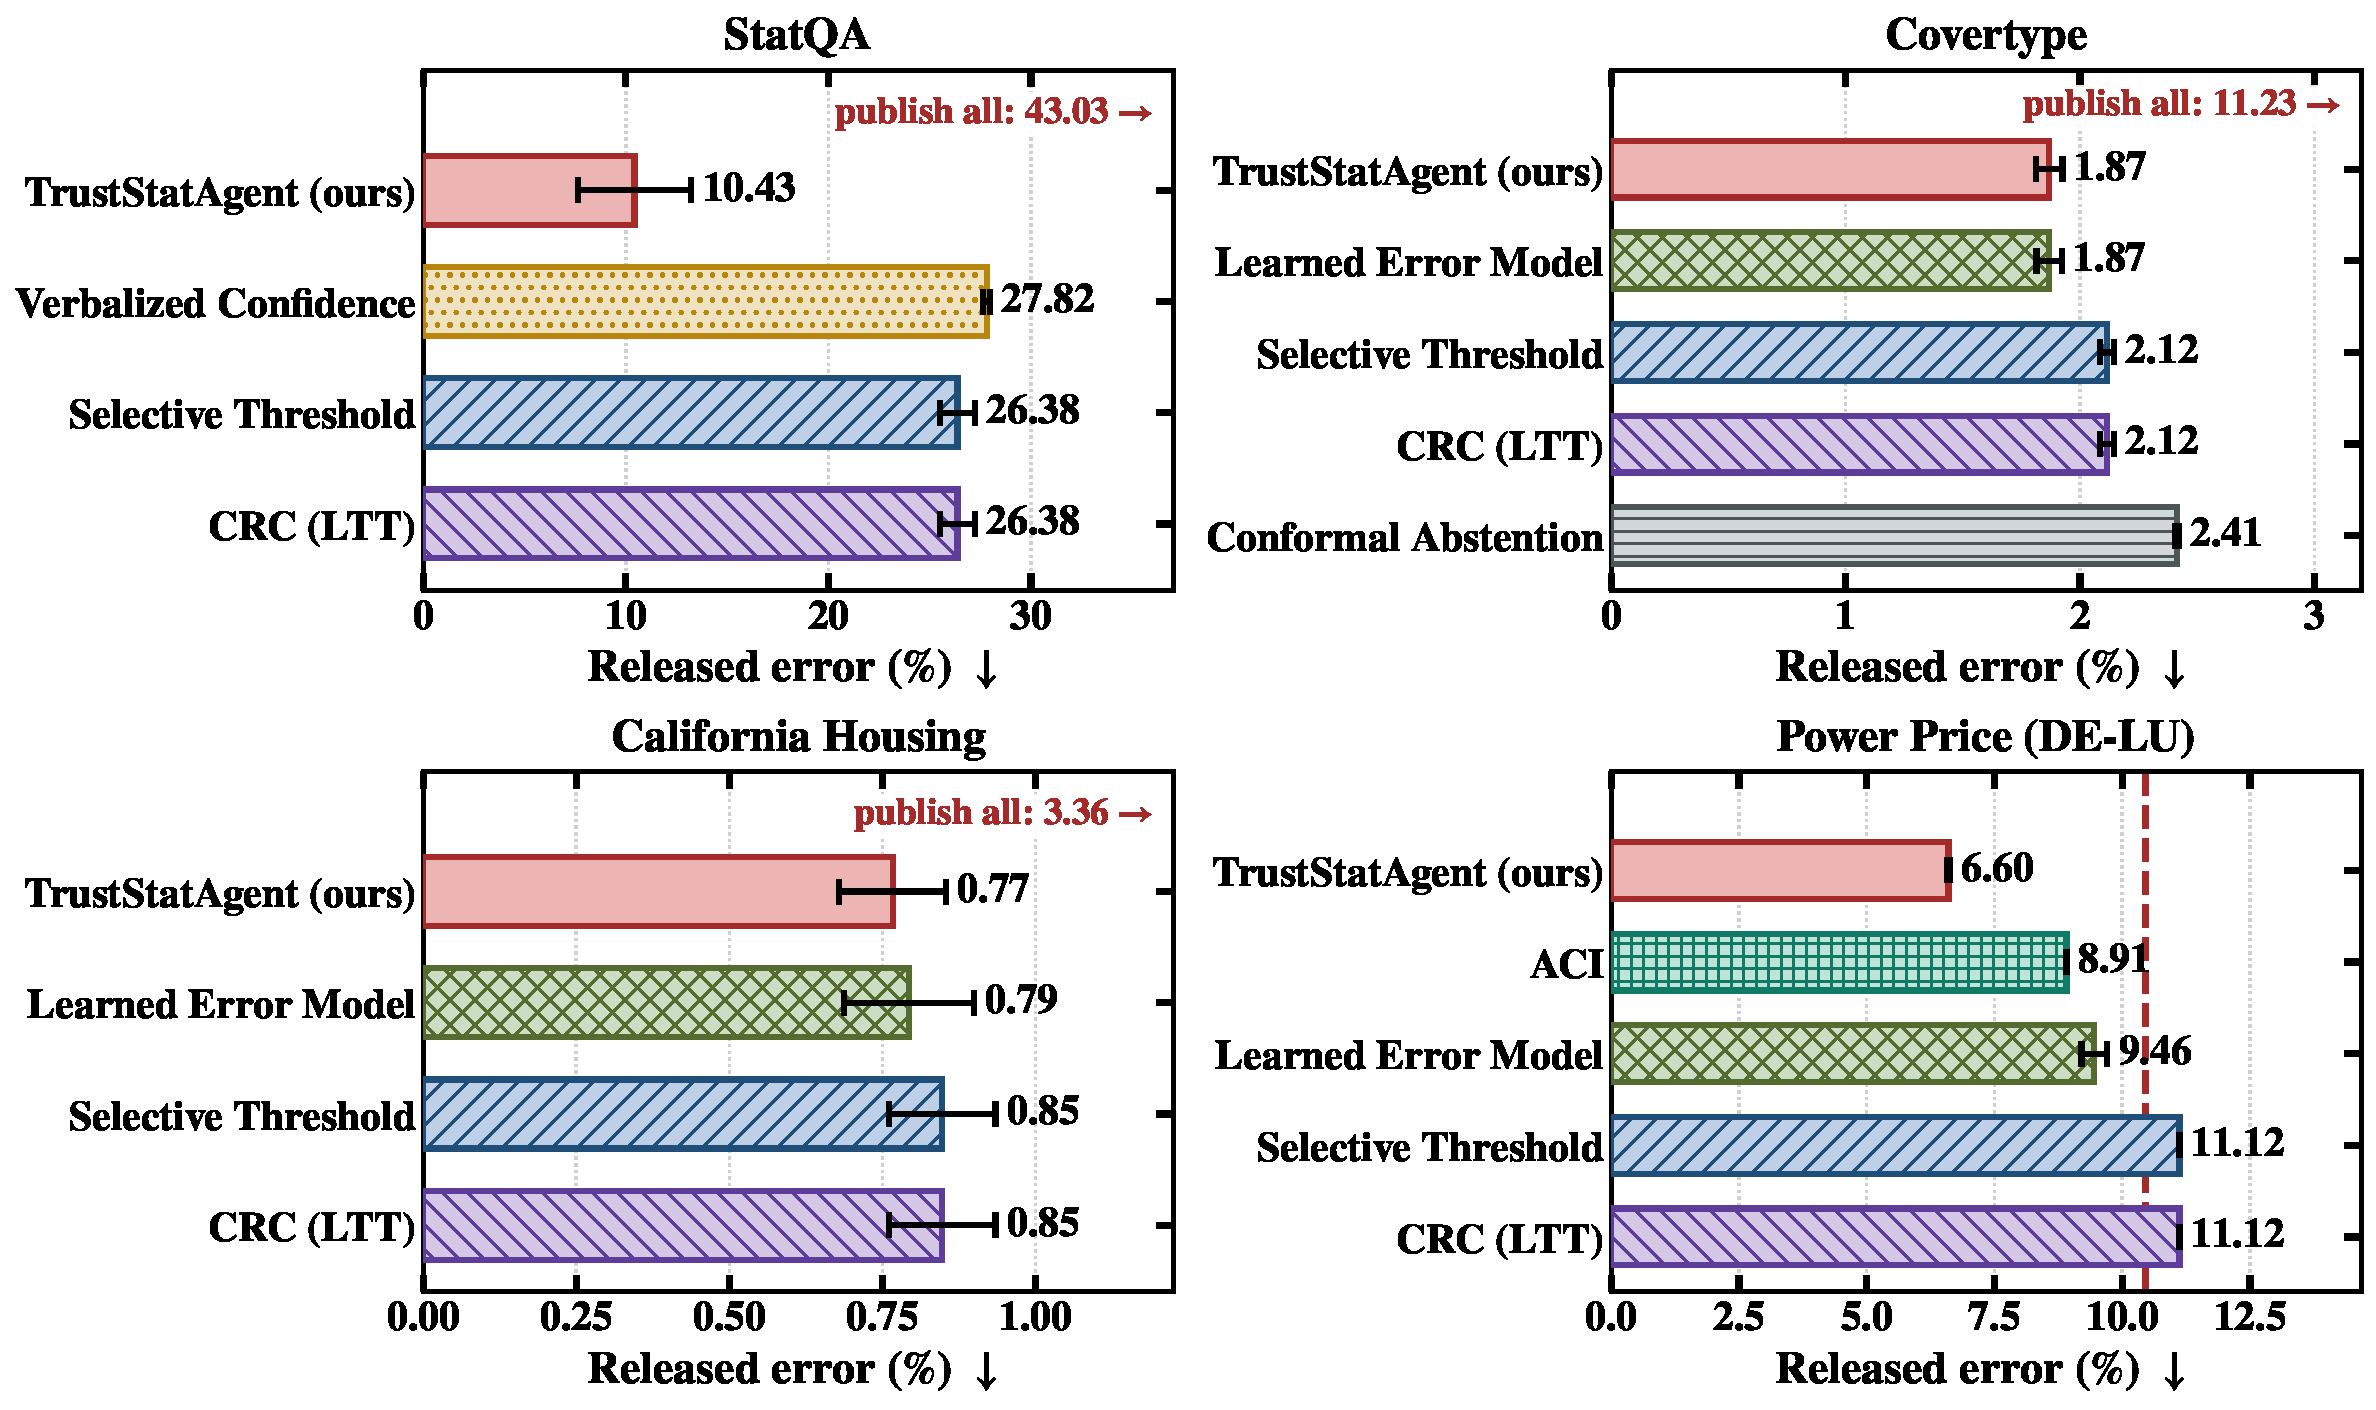
\includegraphics[width=0.98\linewidth]{figures/fig2_main_gating_matrix.pdf}
    \caption{\textcolor{blue}{Released error at the matched 60\% release rate; lower is better. Bars: seed means; error bars: seed s.d. Dashed line: publish-all error of the same candidate pool. Exact values: Table~\ref{tab:matched_release}, 60\% column.}}
    \label{fig:main_gating}
\end{figure}

{\color{blue}
On StatQA TrustStatAgent releases 60\% of candidates at 10.43\% released error, against 26.38\% for selective thresholding and 27.82\% for the model's own verbalized confidence, both significant.
The advantage is largest exactly where single signals carry the least information about correctness.
The gate also adapts its referral behaviour to the difficulty of the task category. It releases \textcolor{red}{86.4}\% of descriptive-statistics candidates, where the pipeline is strong, but only \textcolor{red}{35.4}\% of correlation-analysis candidates, where six in ten candidates are wrong, and the few it releases there are all correct; \ref{app:category} gives the full breakdown.

On Covertype the released error rate is 1.87\%, significantly below both conformal baselines at 2.41\% for abstention and 2.12\% for CRC, and level with the learned error model at 1.87\%. The tie is expected, since that learned error score is itself one of the signals the gate fuses; every result TrustStatAgent releases additionally carries a calibrated interval or set with a 90\% coverage guarantee.

On Power Price the margin is wide and significant against every baseline, at 6.60\% against 8.91\% for ACI, 9.46\% for the learned error model, and 11.12\% for CRC and selective thresholding.
This is the benchmark where the fused signals complement each other most, a point Section~\ref{sec:results_discussion} quantifies.

On California Housing every method releases at an error rate below 1\%, the differences lie within seed noise, and TrustStatAgent matches the strongest baseline at 0.77\% while carrying a coverage certificate the single-signal rules do not provide, with empirical coverage at 90.5\% against the nominal 90\% level.

The end-to-end references mark the alternative to a release layer.
Zero-shot-CoT and ReAct direct produce no per-sample reliability signal, so any deployment of them publishes 100\% of answers at 32.18\% and 44.83\% released error on StatQA; publishing the frozen candidates without a gate costs 43.03\%, 11.23\%, 3.36\%, and 10.46\% on the four benchmarks.

The comparison also exposes the reach of each rule. Verbalized confidence presupposes language-model candidates and appears only on StatQA, conformal abstention presupposes singleton prediction sets, and ACI presupposes a temporal series and appears only on Power Price, so each existing rule leaves a task family in which it defines no release decision at all.
Only selective thresholding, the learned error model, and TrustStatAgent cover all four task families, and only TrustStatAgent adds the calibrated interval or set to every released result.

}

\subsection{The full risk--coverage spectrum}
\label{sec:results_matched}

{\color{blue}
A lead at one release rate could reflect a fortunate threshold rather than a better ranking, so the next question is whether the advantage holds across the whole spectrum. Table~\ref{tab:matched_release} answers it at four matched release rates with AURC as the summary, and Figure~\ref{fig:rc_curves} draws the complete risk--coverage curves.
}

\begin{figure}[H]
    \centering
    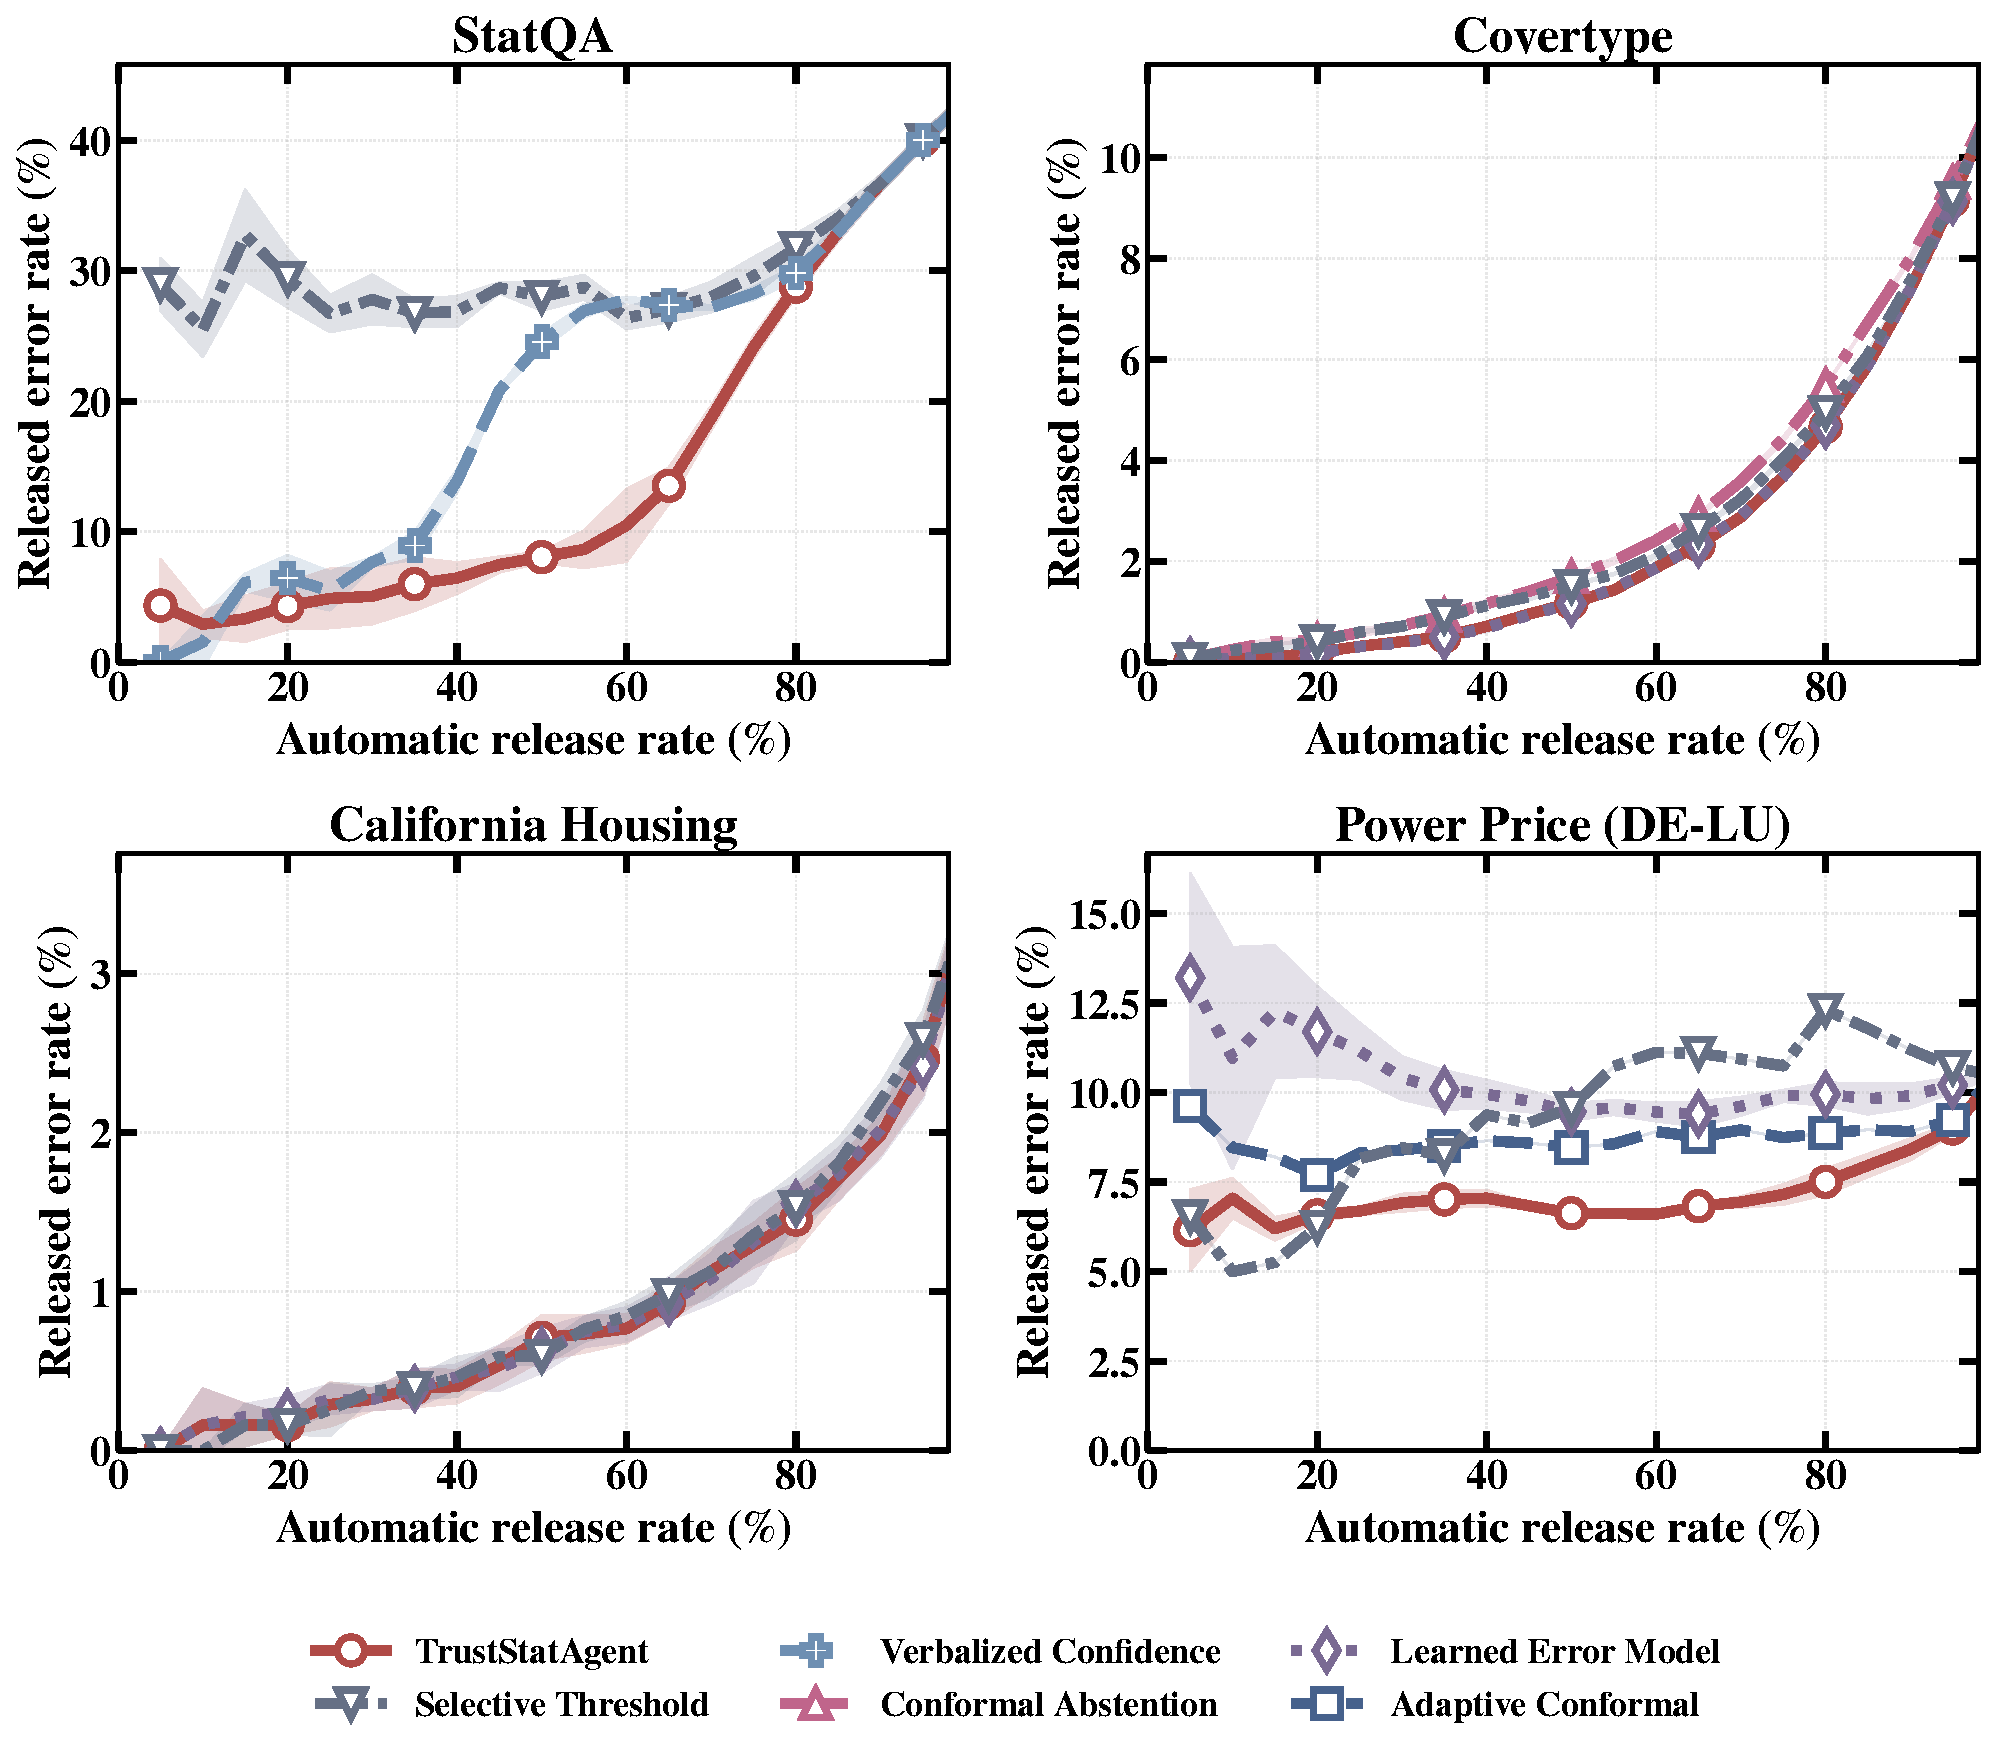
\includegraphics[width=0.74\linewidth]{figures/fig1_rc_curves.pdf}
    \caption{\textcolor{blue}{Risk--coverage curves; lower is better everywhere.}}
    \label{fig:rc_curves}
\end{figure}

\begin{table}[t]
    \centering
    \caption{\textcolor{blue}{Released error (\%) at four matched release rates and AURC ($\times 10^{2}$), means over seeds; lower is better. Bold: best in column block. CRC and selective thresholding share one ranking signal, so their matched rows coincide by construction.}}
    \label{tab:matched_release}
    \scriptsize\color{blue}
    \setlength{\tabcolsep}{4pt}
    \renewcommand{\arraystretch}{1.12}
    \begin{tabular}{@{}llrrrrr@{}}
        \toprule
        \textbf{Benchmark} & \textbf{Method} & \textbf{20\%} & \textbf{40\%} & \textbf{60\%} & \textbf{80\%} & \textbf{AURC} \\
        \midrule
        \multirow{3}{*}{StatQA}
        & \textbf{TrustStatAgent} & \textbf{4.30} & \textbf{6.45} & \textbf{10.43} & \textbf{28.75} & \textbf{14.44} \\
        & Selective threshold     & 29.39 & 26.88 & 26.38 & 31.72 & 29.95 \\
        & Verbalized confidence   & 6.45  & 13.98 & 27.82 & 29.83 & 19.74 \\
        \midrule
        \multirow{5}{*}{Covertype}
        & \textbf{TrustStatAgent} & 0.19 & 0.71 & \textbf{1.87} & \textbf{4.66} & 2.45 \\
        & Learned error model     & \textbf{0.18} & \textbf{0.68} & 1.87 & 4.69 & \textbf{2.45} \\
        & Selective threshold     & 0.41 & 1.12 & 2.12 & 4.95 & 2.70 \\
        & CRC (LTT)               & 0.41 & 1.12 & 2.12 & 4.95 & 2.70 \\
        & Conformal abstention    & 0.43 & 1.16 & 2.41 & 5.48 & 2.91 \\
        \midrule
        \multirow{4}{*}{Calif.\ Housing}
        & \textbf{TrustStatAgent} & \textbf{0.16} & \textbf{0.40} & \textbf{0.77} & \textbf{1.45} & \textbf{0.87} \\
        & Learned error model     & 0.24 & 0.46 & 0.79 & 1.56 & 0.88 \\
        & Selective threshold     & 0.16 & 0.46 & 0.85 & 1.53 & 0.89 \\
        & CRC (LTT)               & 0.16 & 0.46 & 0.85 & 1.53 & 0.89 \\
        \midrule
        \multirow{5}{*}{Power Price}
        & \textbf{TrustStatAgent} & 6.57  & \textbf{7.05} & \textbf{6.60} & \textbf{7.51} & \textbf{7.09} \\
        & ACI                     & 7.69  & 8.65  & 8.91  & 8.87  & 9.01  \\
        & Learned error model     & 11.70 & 9.95  & 9.46  & 9.95  & 10.39 \\
        & Selective threshold     & \textbf{6.25} & 9.38 & 11.12 & 12.31 & 9.71 \\
        & CRC (LTT)               & \textbf{6.25} & 9.38 & 11.12 & 12.31 & 9.71 \\
        \bottomrule
    \end{tabular}
\end{table}


{\color{blue}
The spectrum confirms that the single-point results are structural.
TrustStatAgent attains the lowest AURC on StatQA at 14.44 against 19.74 and 29.95 for the two baselines, on Power Price at 7.09 against 9.01 or higher for every baseline, and on California Housing at 0.87; on Covertype its AURC is statistically indistinguishable from the learned error model's, both at 2.45, and ahead of every conformal baseline.
On StatQA TrustStatAgent is significantly ahead of both baselines at the \textcolor{red}{40\% and 60\%} release rates.
On Power Price it is significantly ahead of all four baselines at 40\%, 60\%, and 80\%; the only point it does not win is the most conservative 20\% corner, where the width-based rules benefit from a handful of extreme forecasts with enormous intervals.
On Covertype it is significantly ahead of the conformal family at all four rates and level with the learned error model throughout.
On California Housing the candidate pool is already so accurate that too few errors remain for any ranking to separate the methods, and we report parity. Section~\ref{sec:results_discussion} turns this floor into a precise statement about when fusion can and cannot add value.

Two features of the curves deserve a direct look.
Verbalized confidence starts competitively on StatQA at 6.45\% released error at the 20\% rate and then collapses to 27.82\% at the 60\% rate. The model knows which of its answers are obviously right but cannot rank the middle of the distribution, which is where a deployment actually operates.
And on Power Price the TrustStatAgent curve is nearly flat between the 40\% and 80\% rates, moving only from 7.05\% to 7.51\%, while every single-signal curve deteriorates, because the rolling-residual and width signals fire on different failure modes and the fusion inherits both.
}

\subsection{Ablation results}
\label{sec:results_ablation}

{\color{blue}
The next question is whether all three modules earn their place or whether one of them does all the work. Table~\ref{tab:ablation_results} removes one module at a time, and Figure~\ref{fig:ablation} summarises the outcome.
}

\begin{figure}[H]
    \centering
    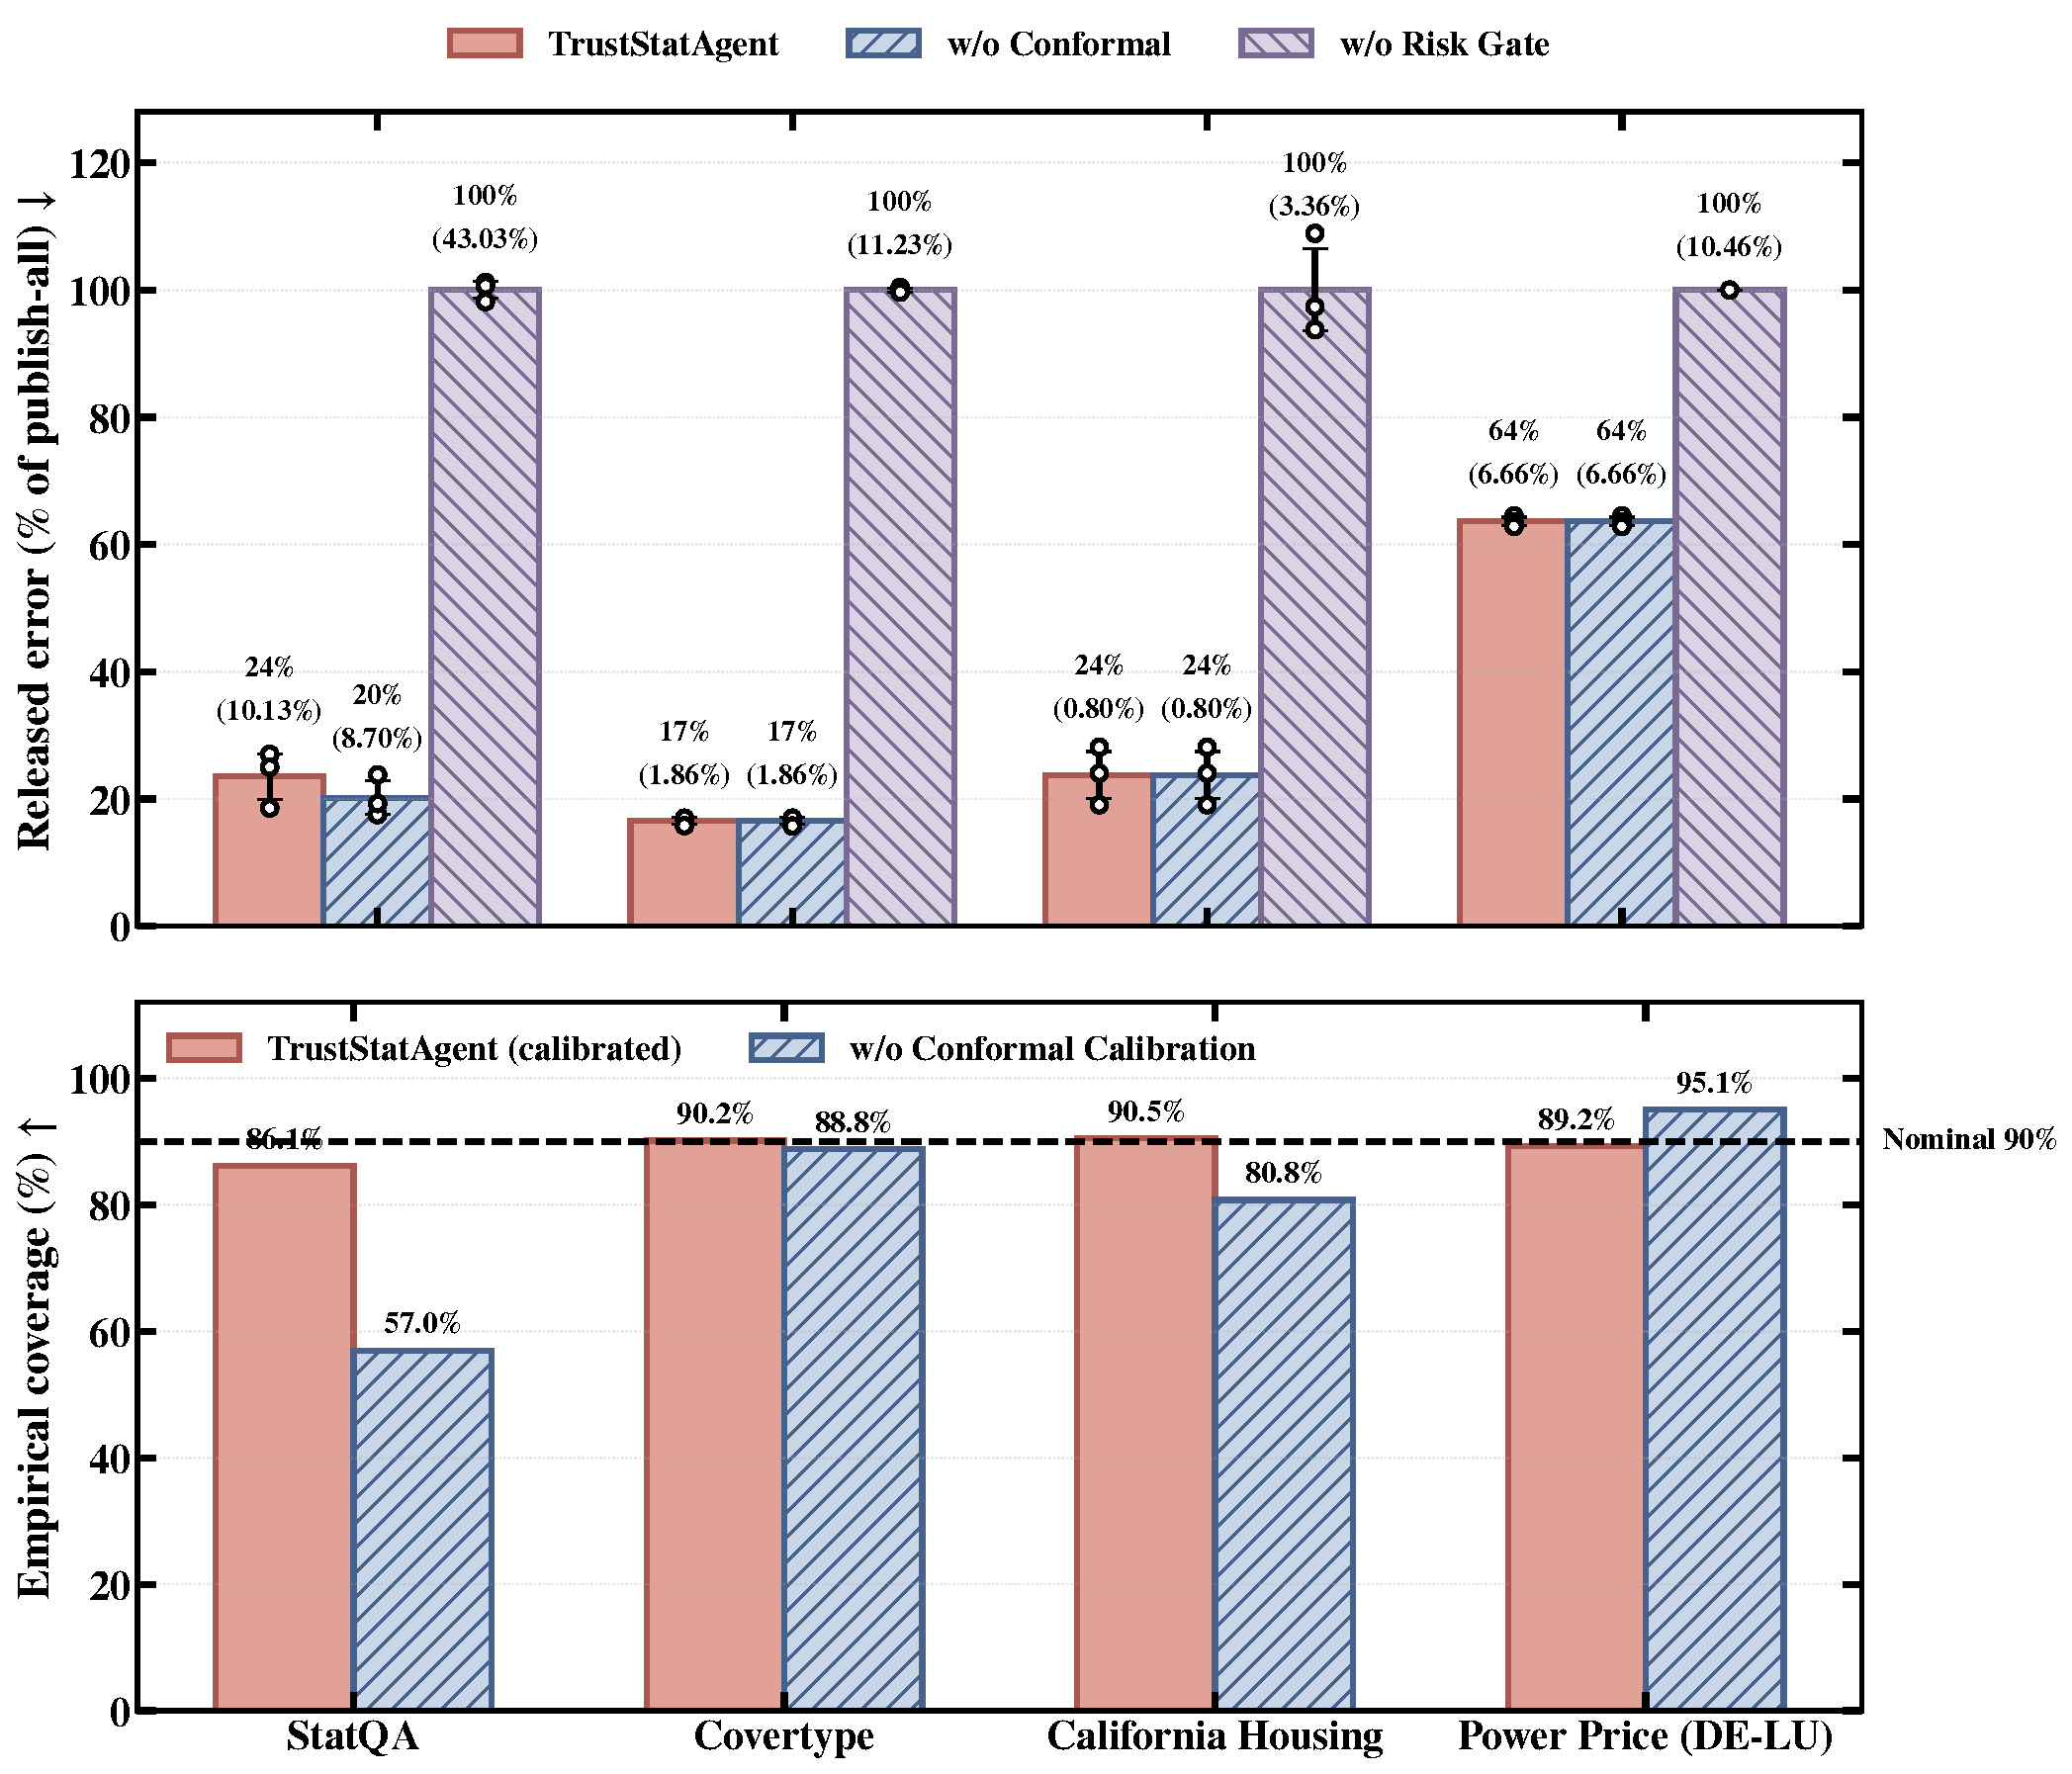
\includegraphics[width=0.74\linewidth]{figures/fig3_ablation.pdf}
    \caption{\textcolor{blue}{Ablation summary. The gate owns the error reduction, calibration owns the certificate, planning owns candidate quality.}}
    \label{fig:ablation}
\end{figure}

\begin{table}[t]
    \centering
    \caption{\textcolor{blue}{Ablations at each variant's natural operating point, mean over seeds. Coverage targets 90\%; StatQA targets no coverage level (---). The planning ablation reports StatQA official accuracy.}}
    \label{tab:ablation_results}
    \scriptsize\color{blue}
    \setlength{\tabcolsep}{4pt}
    \renewcommand{\arraystretch}{1.12}
    \begin{tabular}{@{}llrrr@{}}
        \toprule
        \textbf{Benchmark} & \textbf{Variant} & \textbf{Coverage (\%)} & \textbf{Release (\%)} & \textbf{Rel.\ err.\ (\%)} \\
        \midrule
        \multirow{3}{*}{StatQA}
        & w/o risk gate              & ---   & 100.00 & 43.03 \\
        & w/o conformal calibration  & ---   &  53.88 &  8.70 \\
        & \textbf{Full model}        & ---   &  \textcolor{red}{58.98} &  \textcolor{red}{10.13} \\
        \midrule
        \multirow{3}{*}{Covertype}
        & w/o risk gate              & 90.16 & 100.00 & 11.23 \\
        & w/o conformal calibration  & 88.77 &  59.86 &  1.86 \\
        & \textbf{Full model}        & 90.16 &  59.97 &  1.86 \\
        \midrule
        \multirow{3}{*}{Calif.\ Housing}
        & w/o risk gate              & 80.78 & 100.00 &  3.36 \\
        & w/o conformal calibration  & 80.78 &  60.63 &  0.80 \\
        & \textbf{Full model}        & 90.50 &  60.63 &  0.80 \\
        \midrule
        \multirow{3}{*}{Power Price}
        & w/o risk gate              & 95.08 & 100.00 & 10.46 \\
        & w/o conformal calibration  & 95.08 &  60.96 &  6.66 \\
        & \textbf{Full model}        & 89.23 &  60.96 &  6.66 \\
        \midrule
        \multirow{2}{*}{StatQA}
        & w/o explicit planning (accuracy, \%) & \multicolumn{3}{r}{54.67} \\
        & \textbf{Full model} (accuracy, \%)   & \multicolumn{3}{r}{56.97} \\
        \bottomrule
    \end{tabular}
\end{table}


{\color{blue}
Removing the gate releases every candidate, and the released error rate returns to the candidate error rate of 43.03\% on StatQA, 11.23\% on Covertype, 3.36\% on California Housing, and 10.46\% on Power Price. The entire error reduction of the framework comes from the release decision, none from hiding candidates.

Removing calibration leaves the ranking of candidates in place and therefore leaves the released error rate nearly unchanged at the natural operating point, but it destroys the certificate the framework exists to provide.
Coverage drifts off its nominal 90\% level in both directions, down to 80.78\% on California Housing and up to 95.08\% on Power Price, so the user no longer knows how much trust to place in an interval.
\textcolor{red}{On StatQA the two variants release at similar rates, 58.98\% against 53.88\%, and err within seed noise of each other, 10.13\% against 8.70\%; what calibration adds is again the certificate, with the prediction sets covering 86.1\% of cases against 57.0\% for the uncalibrated variant.}

Removing explicit planning leaves the release layer untouched and damages the input instead. StatQA accuracy falls from 56.97\% to 54.67\%, which confirms that the plan is part of what determines candidate quality, as the autonomous study of Section~\ref{sec:results_autonomous} showed from the other direction.

The three results together exclude the simplest alternative explanation of Figure~\ref{fig:main_gating}, namely that one component does all the work. The gate owns the error reduction, calibration owns the certificate, and planning owns candidate quality.
}

\subsection{Generality across language-model backbones}
\label{sec:results_multillm}

{\color{blue}
The main experiments use GPT-6.1-sol. To check that \textcolor{red}{the framework} transfers across backbones, we repeat the StatQA comparison with three further models from different providers and families --- Qwen3.7-Max (Alibaba), GLM-5.3 (Zhipu AI), and Grok-4.7 (xAI) --- under an identical protocol. StatQA is the natural test bed for this check, as the only benchmark whose candidates are written by the language model itself; on the predictive benchmarks the candidates come from statistical tools, so a backbone swap changes little there. Calibration and gating make no language-model calls, so only the candidate pools differ; backbone execution failures are intercepted as non-release, and all rates are computed on the valid candidates.

\textcolor{red}{Table~\ref{tab:multillm} shows that the gain transfers to every backbone: at the 60\% release target the gate errs at 10.1--23.5\%, against 43.0--53.9\% for publishing every candidate and 25.2--31.7\% for the strongest baseline, and below selective thresholding at \textcolor{red}{45 of the 48 combinations of backbone, split seed, and release rate and never above it} (Figure~\ref{fig:multillm}).}
}

\begin{table}[t]
    \centering
    \caption{\textcolor{blue}{Cross-backbone results on StatQA at the 60\% release target (mean over three seeds); lower is better. \textcolor{red}{``Best base.'': the stronger of selective thresholding and verbalized confidence at the matched release rate.}}}
    \label{tab:multillm}
    \scriptsize\color{blue}
    \setlength{\tabcolsep}{3.5pt}
    \renewcommand{\arraystretch}{1.15}
    \resizebox{\linewidth}{!}{%
    \begin{tabular}{@{}lcccccc@{}}
        \toprule
        \textbf{Backbone} & \textbf{Acc.\ (trust)} & \textbf{Acc.\ (ZS-CoT)} & \textbf{No-gate err.} & \textbf{Gated err.} & \textbf{Release} & \textbf{Best base.} \\
        & (\%) & (\%) & (\%) & (\%) & (\%) & (\%) \\
        \midrule
        GPT-6.1-sol & 57.0 & \textcolor{red}{67.8} & 43.0 & \textcolor{red}{\textbf{10.1}} & \textcolor{red}{59.0} & 26.4 \\
        Qwen3.7-Max & 46.1 & 57.8 & 53.9 & \textcolor{red}{\textbf{23.5}} & \textcolor{red}{58.8} & 31.7 \\
        GLM-5.3     & 49.6 & \textcolor{red}{55.5} & 50.4 & \textcolor{red}{\textbf{21.1}} & \textcolor{red}{59.2} & 28.5 \\
        Grok-4.7    & 49.9 & \textcolor{red}{65.1} & 50.1 & \textcolor{red}{\textbf{20.8}} & \textcolor{red}{61.1} & 25.2 \\
        \bottomrule
    \end{tabular}}
\end{table}

\begin{figure}[H]
    \centering
    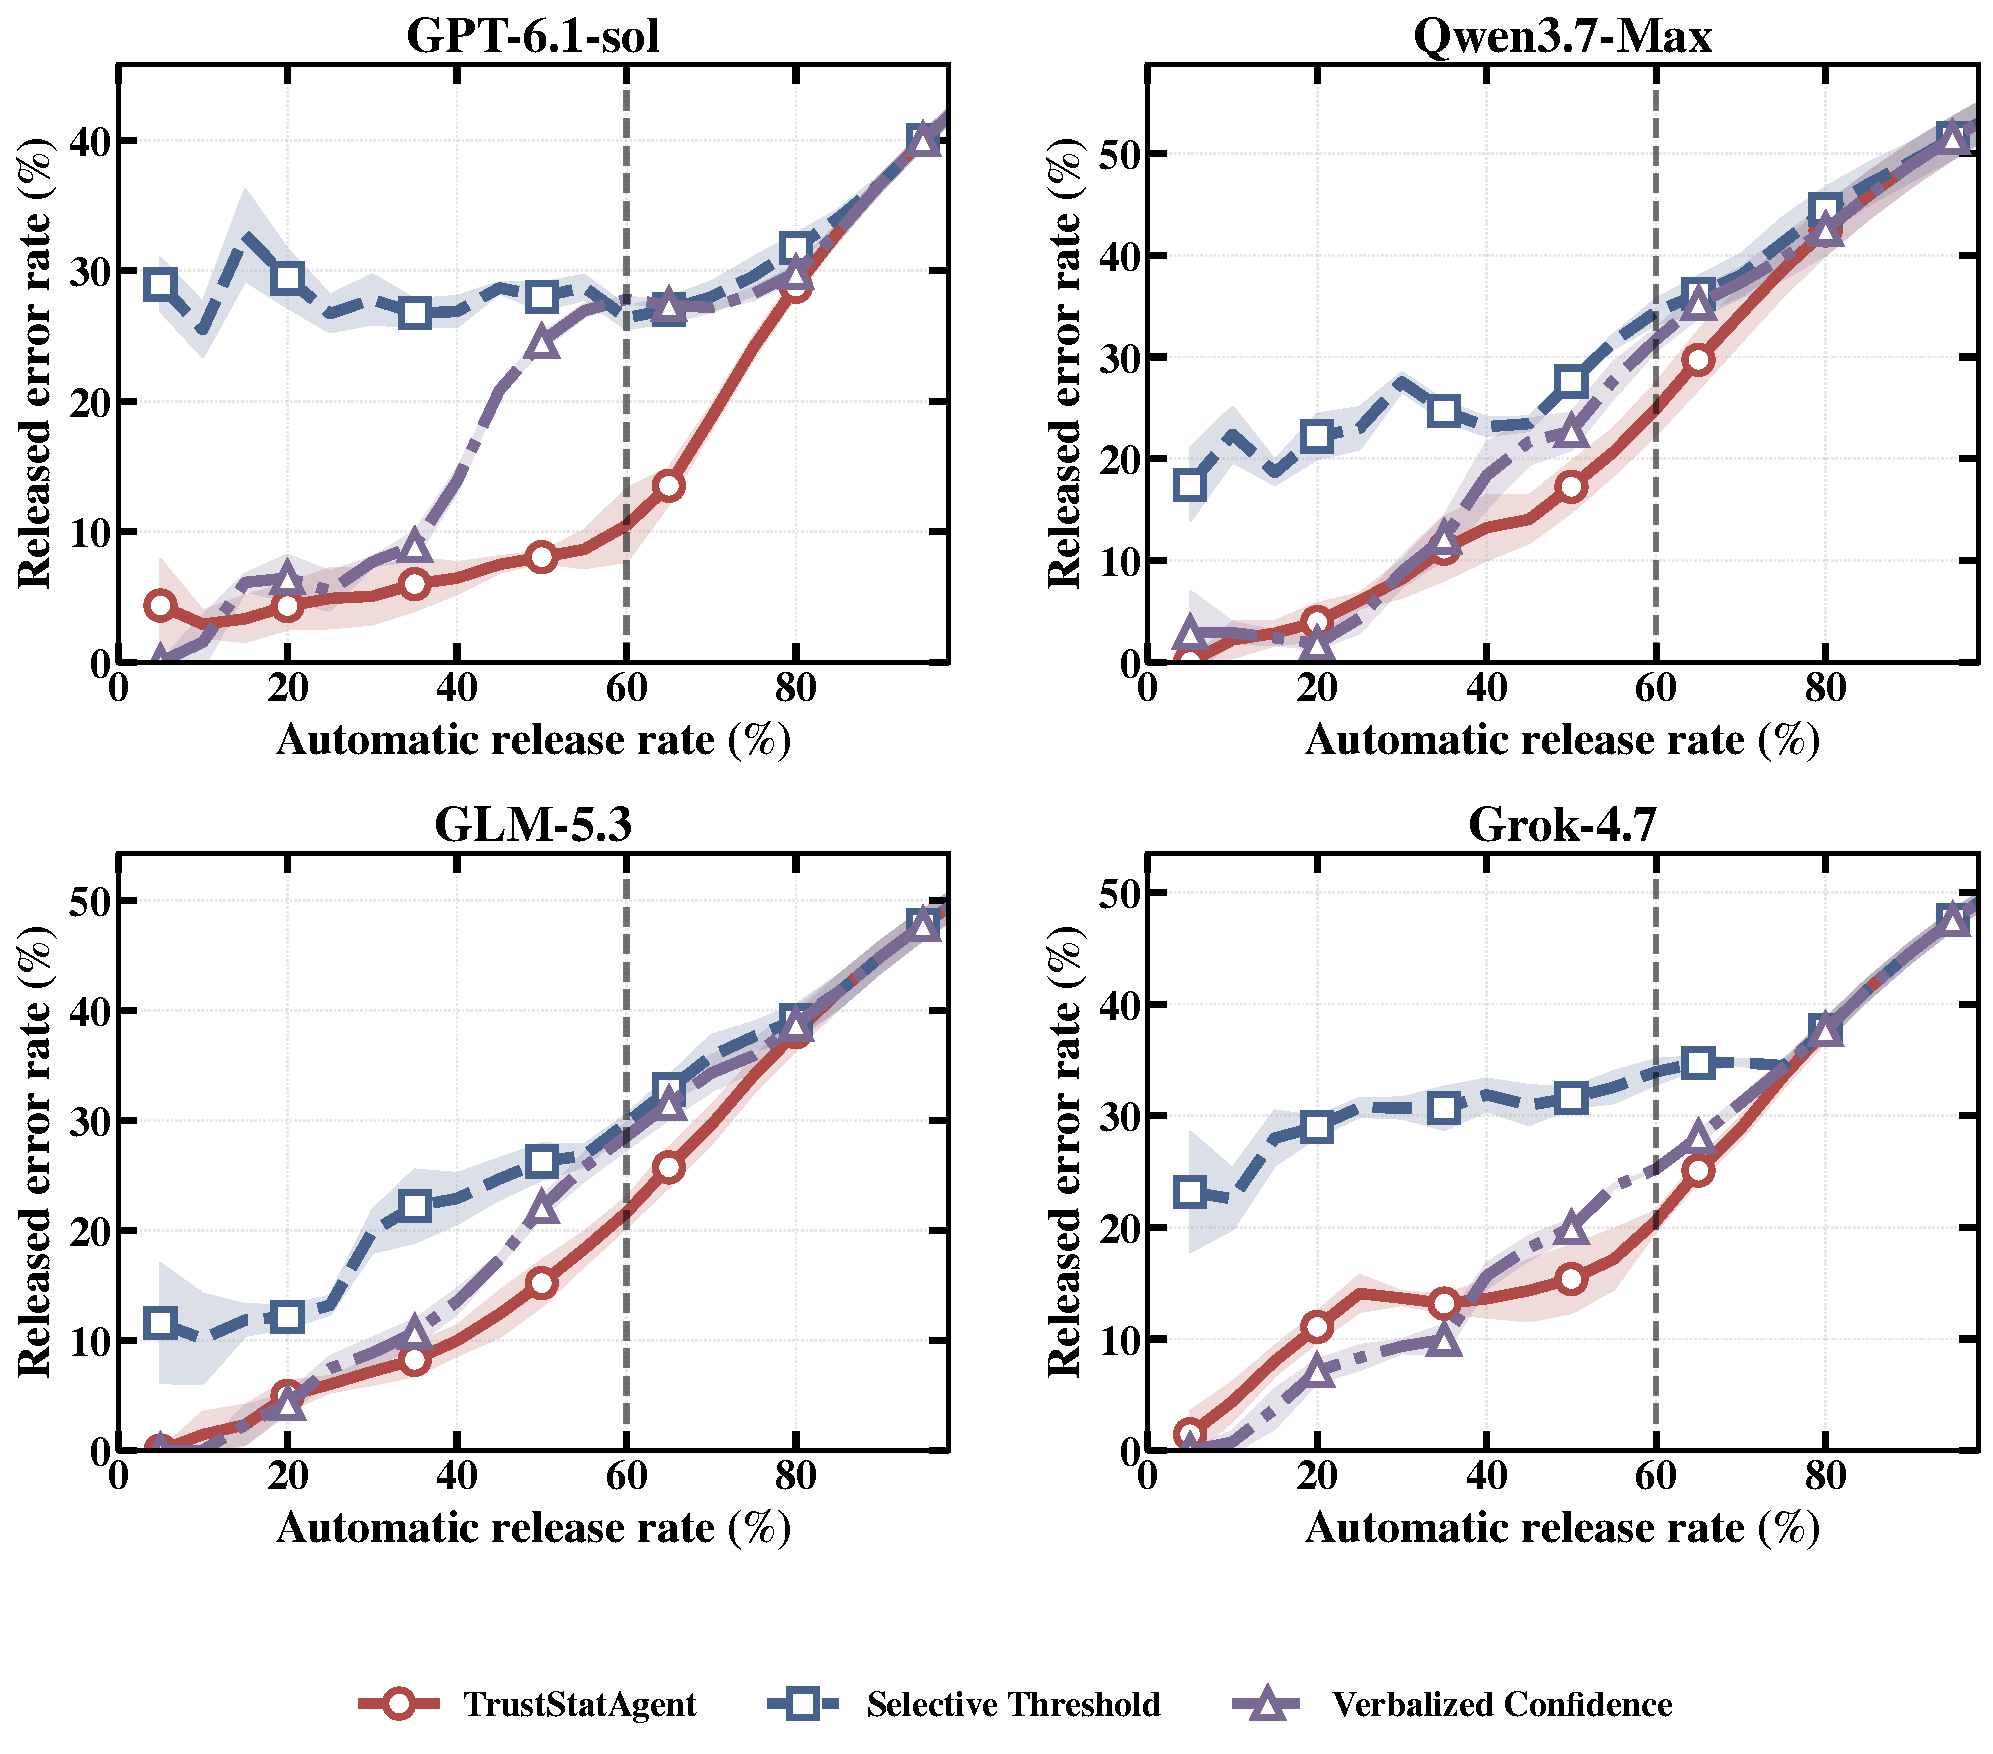
\includegraphics[width=0.9\linewidth]{figures/fig5_multillm.pdf}
    \caption{\textcolor{red}{Risk--coverage curves on StatQA across the four backbones (mean over three seeds; shading: s.d.). Dashed line: the 60\% release target reported in Table~\ref{tab:multillm}.}}
    \label{fig:multillm}
\end{figure}

\section{Discussion}
\label{sec:results_discussion}

{\color{blue}
Sections~\ref{sec:results_release} and~\ref{sec:results_matched} read the results one benchmark at a time; reading them together answers two questions, when fusing several signals beats the best single one, and what the release layer costs to operate.
The first question is about our own design: the risk gate ranks candidates by fusing several calibrated signals, interval width, a learned error score, rolling residuals, and answer agreement, while every compared baseline ranks by a single one.

\begin{enumerate}
    \renewcommand{\labelenumi}{\color{blue}\arabic{enumi}.}
    \setlength{\itemsep}{5pt}

    \item \textbf{Fusion pays exactly when candidate errors scatter across signals.}
    California Housing supplies the boundary case: its pool is already so accurate, 3.36\% base error, that too few violations remain for any ranking to exploit, every method releases below 1\%, and parity is the correct outcome rather than a missing result.
    Where errors scatter across signals, fusion wins clearly: AURC 7.09 against 9.01 for the best single-signal rule on Power Price, a 21\% reduction, and 14.44 against 19.74 on StatQA, a 27\% reduction.
    Where one signal already identifies the errors, fusion has nothing left to add: on Covertype the learned error score is one of the fused components, and the gate matches it at 2.45, so the differentiator there is the 90\% coverage certificate.
    A deployment can diagnose its own regime on validation data in advance, by checking whether its candidate errors concentrate under one signal or scatter across several.

    \item \textbf{The exchange is affordable under modest cost assumptions.}
    Writing $c_e$ for the cost of a published violation and $c_r$ for the cost of one referral, the expected cost per candidate is proportional to $\rho\,r\,e+(1-r)$ with $\rho=c_e/c_r$, and the gated policy beats publishing everything once $\rho$ exceeds $\rho^{\ast}=(1-r)/(p-r\,e)$: \textcolor{red}{1.1} on StatQA, 4.0 on Covertype, 6.1 on Power Price, and 13.7 on California Housing (Fig.~\ref{fig:cost_ratio}).
    Where violations are common, a published error need only cost a few times a referral for the gate to pay for itself; where they are rare the argument requires an order of magnitude more, because most referrals are then unnecessary.
    The referral load an operator would size review capacity against is \textcolor{red}{41.0}\% of candidates on StatQA, 40.0\% on Covertype, 39.4\% on California Housing, and 39.0\% on Power Price.
\end{enumerate}

Two further observations merit emphasis.
Our agent earns its place exactly where the fixed pipeline is wrong, lifting Covertype accuracy from 0.697 to 0.887 by replacing the author-chosen logistic regression, and our gate removes 58\% to 83\% of the released error \textcolor{red}{across the autonomous arms}.
In our design the release decision belongs to a deterministic program rather than to the model's self-report. The program's inputs are inspectable, and because our calibration never touches the generator, our release layer transfers unchanged across backbones (Section~\ref{sec:results_multillm}).
Against selective-prediction and conformal language-modelling work~\citep{geifman2017selective,elyaniv2010foundations,lee2024selective,quach2024conformal,wang2024conu,cherian2024large}, our difference lies in what is calibrated, a computational result whose execution is also checked, so our rule covers all four task families whereas every compared rule leaves at least one family undefined.
}

\begin{figure}[t]
    \centering
    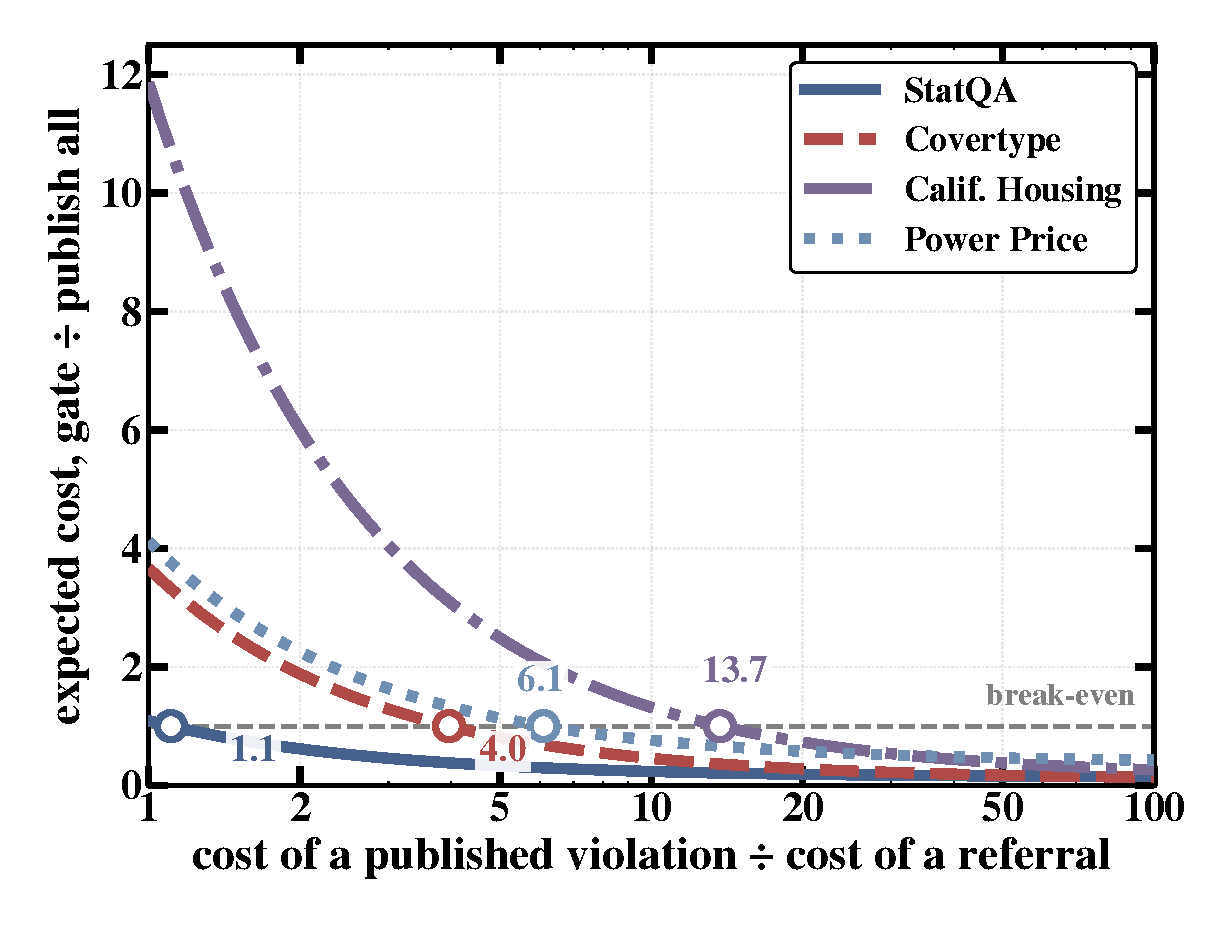
\includegraphics[width=0.72\linewidth]{figures/fig_cost_ratio.pdf}
    \caption{\textcolor{blue}{Relative expected cost of the gated policy against publishing everything as a function of the cost ratio $\rho=c_e/c_r$ (logarithmic axis); $r$ and $e$ from Table~\ref{tab:ablation_results}, $p$ the candidate error rate. Circles mark the break-even ratios quoted in the text.}}
    \label{fig:cost_ratio}
\end{figure}


\section{Conclusion}
\label{sec:conclusion}

{\color{blue}
This paper addressed the point at which a statistical agent stops producing a result and starts publishing one.
The difficulty lies outside computation, since a tool can fit a model and a language model can plan which model to fit.
An uncalibrated confidence score gives no finite-sample basis for deciding whether a particular result is safe to release, and a reliability criterion taken alone can be satisfied by publishing nothing.
We therefore treated statistical accuracy and publishing reliability as a joint objective and proposed TrustStatAgent.
A tool-restricted LLM agent produces candidates, conformal calibration attaches a coverage statement to each candidate, and a deterministic risk gate releases only those results whose execution is compliant and whose calibrated output lies inside the task's acceptance region.
Release authority is separated from generation, so the model that produces a number does not decide whether the number is published.

The experiments support the design on four benchmarks.
Left to plan for itself, the agent selects methods that beat a fixed reference pipeline, most sharply on Covertype, where accuracy rises from 0.697 to 0.887, and a failure-injection probe confirms that every corrupted tool call is intercepted before release.
Against publishing every candidate from the same pipeline, the gate reduces the released error rate from 43.03\% to \textcolor{red}{10.13}\% on StatQA, from 11.23\% to 1.86\% on Covertype, from 3.36\% to 0.80\% on California Housing, and from 10.46\% to 6.66\% on Power Price, at release rates of \textcolor{red}{59}\% to 61\%.
Compared at identical release rates, TrustStatAgent attains a risk--coverage area that is the lowest or statistically indistinguishable from the lowest on every benchmark, and every released result additionally carries a 90\% coverage certificate that the single-signal rules do not provide.
The ablations assign each module its own job, the gate the error reduction, calibration the certificate, and planning the candidate quality, and the release layer itself makes no language-model calls and transfers unchanged across three further model families, where it cuts the released error of the noisiest candidate pool from 53.9\% to \textcolor{red}{23.5}\%.

Three extensions follow.
First, the exchangeability assumption should be replaced by online calibration for the forecasting task and by stratified calibration for heterogeneous item pools, so that the guarantee applies to the units on which the decision is actually taken.
Second, the operating point should follow from a stated cost ratio rather than a fixed tolerance, and the referral should distinguish degrees of review beyond the present two levels.
Third, the workflow should be tested on tasks whose correctness depends on several modelling decisions at once, such as model diagnostics and multiple-testing corrections, where the acceptance region is harder to specify than an error band but where the same separation between generation and release applies.
}


\section*{CRediT authorship contribution statement}
\textbf{Yifei Gao}: Methodology, Investigation, Writing -- original draft.
\textbf{Jintian Qian}: Visualization, Writing -- original draft.
\textbf{Jiayi Wang}: Writing -- original draft.
\textbf{Zhuang Liu}: Supervision, Writing -- review \& editing.

\section*{Declaration of Competing Interest}
The authors declare that they have no known competing financial interests or personal relationships that could have appeared to influence the work reported in this paper.

\section*{Funding}
This research did not receive any specific grant from funding agencies in the public, commercial, or not-for-profit sectors.

\section*{Data availability}
The complete implementation of TrustStatAgent, including the evaluation pipelines, the frozen StatQA candidate outputs, the multi-seed evaluation scripts, and the configuration files underlying every reported figure, is publicly available at \url{https://github.com/Yifei-create/TrustStatAgent}.

\appendix

\section{Raw confusion counts}
\label{app:counts}

\begin{table}[H]
    \centering
    \caption{Confusion matrix for release decisions.}
    \label{tab:exp_release_confusion}
    \small
    \renewcommand{\arraystretch}{1.2}
    \begin{tabularx}{\linewidth}{
        @{}
        >{\raggedright\arraybackslash}p{0.26\linewidth}
        >{\raggedright\arraybackslash}X
        >{\raggedright\arraybackslash}X
        @{}
    }
        \toprule
        \textbf{System decision}
        & \textbf{Actual error}
        & \textbf{Actual correct} \\
        \midrule
        Referred for review
        & TP: error intercepted
        & FP: correct result withheld \\
        Automatically released
        & FN: error released
        & TN: correct result retained \\
        \bottomrule
    \end{tabularx}
\end{table}



{\color{blue}
Table~\ref{tab:raw_counts} reports the raw integer counts behind the release statistics of Sections~\ref{sec:results_release} and~\ref{sec:results_ablation}, following the convention of Table~\ref{tab:exp_release_confusion}: an actual error is the positive class and referral for review is the positive decision, so TP denotes an intercepted error, FN a released error, TN a correct result released, and FP a correct result withheld.
The counts correspond to the reference seed 42 at each policy's natural operating point; the matched-release comparisons of Sections~\ref{sec:results_release} and~\ref{sec:results_matched} re-rank the same candidates, and the per-seed counts are included in the code repository.
The true labels enter only after every release decision has been fixed, to score the decisions; they are never available to the gate itself.
}

\begin{table}[H]
    \centering
    \caption{\textcolor{blue}{Raw confusion counts on the test partitions at the reference seed, each policy at its natural operating point. StatQA has 464 test items, Covertype 20{,}000, California Housing 4{,}128, and Power Price 5{,}200.}}
    \label{tab:raw_counts}
    \footnotesize\color{blue}
    \setlength{\tabcolsep}{7pt}
    \renewcommand{\arraystretch}{1.12}
    \begin{tabular}{@{}llrrrr@{}}
        \toprule
        \textbf{Benchmark} & \textbf{Policy} & \textbf{TP} & \textbf{FN} & \textbf{TN} & \textbf{FP} \\
        \midrule
        StatQA & TrustStatAgent & \textcolor{red}{172} & \textcolor{red}{30} & \textcolor{red}{228} & \textcolor{red}{34} \\
               & Selective threshold & \textcolor{red}{104} & \textcolor{red}{98} & \textcolor{red}{235} & \textcolor{red}{27} \\
               & Verbalized confidence & \textcolor{red}{125} & \textcolor{red}{77} & \textcolor{red}{203} & \textcolor{red}{59} \\
               & w/o conformal calibration & 177 & 25 & 219 & 43 \\
               & w/o risk gate & 0 & 202 & 262 & 0 \\
               & ReAct direct & 0 & 216 & 248 & 0 \\
               & Zero-shot-CoT & 0 & 148 & 316 & 0 \\
        \midrule
        Covertype & TrustStatAgent & 2{,}029 & 227 & 11{,}776 & 5{,}968 \\
              & Selective threshold & 1{,}994 & 262 & 11{,}803 & 5{,}941 \\
              & Conformal abstention & 494 & 1{,}762 & 17{,}216 & 528 \\
              & CRC (LTT) & 1{,}242 & 1{,}014 & 15{,}858 & 1{,}886 \\
              & w/o conformal calibration & 2{,}029 & 227 & 11{,}745 & 5{,}999 \\
              & w/o risk gate & 0 & 2{,}256 & 17{,}744 & 0 \\
        \midrule
        Calif. Housing & TrustStatAgent & 131 & 20 & 2{,}454 & 1{,}523 \\
              & Selective threshold & 127 & 24 & 2{,}475 & 1{,}502 \\
              & w/o risk gate & 0 & 151 & 3{,}977 & 0 \\
        \midrule
        Power Price & TrustStatAgent & 329 & 215 & 2{,}971 & 1{,}685 \\
              & Selective threshold & 23 & 521 & 4{,}060 & 596 \\
              & ACI & 250 & 294 & 3{,}060 & 1{,}596 \\
              & CRC (LTT) & 514 & 30 & 584 & 4{,}072 \\
              & w/o risk gate & 0 & 544 & 4{,}656 & 0 \\
        \bottomrule
    \end{tabular}
\end{table}

{\color{blue}
Two features of the table are worth reading directly.
On Power Price, selective thresholding and conformal risk control rank candidates by the same signal yet land on opposite ends of the automation scale, releasing 88.1\% of candidates at 11.4\% released error and 11.8\% at 4.9\%; the matched-release protocol of Section~\ref{sec:evaluation_protocol} exists precisely to remove this threshold arbitrariness from the comparison.
\textcolor{red}{On StatQA the verbalized-confidence gate releases 60.3\% of candidates at its natural operating point and errs at 27.5\%, essentially its matched-release row; its failure is therefore ranking quality rather than timidity.}
Removing calibration leaves the released set untouched on California Housing and Power Price, identical TP, FN, TN, and FP rows to the full model, and only moves empirical coverage off its nominal level, so those rows are omitted.
The StatQA counts of CRC are omitted on the same ground of redundancy: its matched-release rows coincide with selective thresholding by construction (Section~\ref{sec:comparative_methods}), and its natural operating point would add only the cross-operating-point comparison that the matched-release protocol exists to remove.
The Power Price CRC row is retained because there the contrast between two natural operating points of one shared ranking is itself the evidence for the protocol.
}

\section{Prompts}
\label{app:prompts}

{\color{blue}
All calls use the configuration of Section~\ref{sec:llm_configuration}.
The system prompt of the planning agent is reproduced verbatim below; it is identical across the four benchmarks, and the per-benchmark task constraints that accompany it in the user prompt follow in the second box.
}

\begin{promptbox}{System prompt, planning agent}
You are the TrustStat statistical analysis agent. You plan and execute
statistical analyses by calling authorized Python tools, and you return one
valid JSON object per step. All numerical computation, model fitting, and
prediction is performed by the tools. Use no unstated numerical claims. Do
not return Markdown or commentary.

Follow this procedure strictly:

\textbf{\textrm{Step 1 --- Inspect.}} Call the authorized inspection tool on the authorized
data identifier. Note variable types, scale, missing values, and
distributional properties relevant to the task.

\textbf{\textrm{Step 2 --- Compare.}} When the task involves choosing among models or methods,
call the authorized comparison or validation tools on at least two
candidates from the authorized whitelist BEFORE choosing. Base the final
choice on this evidence, not on prior preference.

\textbf{\textrm{Step 3 --- Plan.}} Emit a structured plan with exactly these keys: task\_type,
target, selected\_variables, method, preprocessing, tool\_sequence. The
method must be exactly one authorized method name (or a list of authorized
statistical method names when the task requires method selection), with no
explanation embedded. The tool\_sequence must list the tools you actually
call.

\textbf{\textrm{Step 4 --- Execute.}} Call the authorized tools according to the plan.

\textbf{\textrm{Step 5 --- Answer.}} Return the final candidate together with your calibrated
self-assessed confidence in [0,1] that the candidate is fully correct.

Constraints:

-- Use only the authorized data identifiers and only the authorized tools.
Test labels are never available and must never be requested.

-- A plan emitted without a completed Step 2 comparison is invalid when a
comparison tool is available.

-- Choose methods whose assumptions match the VERIFIED data characteristics
(e.g., Fisher Exact Test instead of Chi-square for small expected counts;
Spearman instead of Pearson for non-linear monotone relations).

-- Do not invent metrics, scores, or predictions; only tool observations are
valid evidence.

-- Every response is exactly one JSON object with keys: plan (when emitting
or updating the plan), tool (name or null), arguments (object), candidate
(object or null; only at the final step), confidence (number in [0,1],
required with candidate).
\end{promptbox}

{\color{blue}
The user prompt is a JSON object containing the task specification, the authorized data identifiers, the allowed tools with their contracts, the accumulated tool observations, and a task-constraints block that pins the target and method whitelist of each benchmark.
}

\begin{promptbox}{Task constraints, per benchmark}
\textbf{\textrm{California Housing:}} Set target exactly to MedHouseVal and method exactly to
one of the authorized regression model names; do not put explanations or
provisional wording in the method field. Your plan will be checked for a
completed inspect-and-compare step before model selection.

\textbf{\textrm{Covertype:}} Set target exactly to cover\_type and method exactly to one of
the authorized classification model names; the same inspect-and-compare
check applies.

\textbf{\textrm{Power Price:}} Set target exactly to price and method exactly to one of the
authorized regression model names; the target is 24 hours ahead; compare
models using chronological cross-validation with a 24-row gap, and never use
residuals until their outcomes have been observed.

\textbf{\textrm{StatQA:}} Call inspect\_column\_stats on the authorized data table with the
candidate columns before answering. Each method must be exactly one name
from the method\_catalog in metadata; a list of applicable methods is
allowed. Base method choice on the verified column statistics (types,
missingness, expected cell counts, correlation).
\end{promptbox}

{\color{blue}
The baseline and ablation variants replace only the system prompt and leave the task inputs and the tool budget unchanged.
The verbalized-confidence baseline requires no separate elicitation: it reads the confidence value that Step 5 of the system prompt already returns with every candidate.
The correctness scorer used for calibration on StatQA is a TF--IDF logistic regression (Section~\ref{sec:execution}) and involves no language-model call.
}

\begin{promptbox}{Baseline and ablation system prompts}
ReAct direct: Use an interleaved Thought--Action--Observation protocol.
Call only authorized tools and return JSON. Do not decide publication.

Without explicit planning: Call authorized statistical tools directly to
complete the task. Return JSON and do not decide publication.

Zero-shot-CoT: Think step by step and answer in JSON. Do not call tools.
\end{promptbox}

\section{Computational budget}
\label{app:budget}

{\color{blue}
The data partitioning of every benchmark is given in Section~\ref{sec:benchmark_tasks}.
The language-model budget of the full evaluation is modest.
On StatQA, four candidate pipelines (TrustStatAgent, ReAct direct, Zero-shot-CoT, and the without-planning ablation) each process the 1{,}163 items; TrustStatAgent and ReAct run as multi-step loops capped at eight calls per item, while the verbalized-confidence baseline reuses the self-assessment returned with each candidate and adds no calls.
The autonomous study of Section~\ref{sec:results_autonomous} runs 20 tasks per benchmark and seed with two planning arms, 360 agent runs in total averaging about four calls each; the fixed arms make no language-model calls.
The cross-backbone study repeats one TrustStatAgent pass and one Zero-shot-CoT pass per additional backbone over the same 1{,}163 StatQA items.
All remaining computation is performed by the fixed statistical pipelines and involves no language-model calls.
}

\section{Per-category behaviour on StatQA}
\label{app:category}

{\color{blue}
Table~\ref{tab:statqa_categories} decomposes the StatQA results of Section~\ref{sec:results_release} by task category, pooled over the three split seeds.
\textcolor{red}{The gate releases over 80\% of candidates in the two strongest categories and refers the majority of the three hardest ones, where the released error rate stays below 1\% in two of them.}
}

\begin{table}[H]
    \centering
    \caption{\textcolor{blue}{Per-category behaviour of TrustStatAgent on the StatQA test partitions, pooled over the three split seeds (1{,}392 items). Released error rate is computed within the released subset of each category.}}
    \label{tab:statqa_categories}
    \small\color{blue}
    \setlength{\tabcolsep}{7pt}
    \renewcommand{\arraystretch}{1.15}
    \begin{tabular}{@{}lrrrr@{}}
        \toprule
        \textbf{Task category} & \textbf{$n$} & \textbf{Acc. (\%)} & \textbf{Rel. (\%)} & \textbf{Rel. err. (\%)} \\
        \midrule
        Contingency Table Test & 309 & 70.6 & \textcolor{red}{82.5} & \textcolor{red}{17.6} \\
        Correlation Analysis & 198 & 40.4 & \textcolor{red}{35.4} & \textcolor{red}{0.0} \\
        Descriptive Statistics & 309 & 81.6 & \textcolor{red}{86.4} & \textcolor{red}{5.6} \\
        Distribution Compliance Test & 285 & 39.6 & \textcolor{red}{40.0} & \textcolor{red}{0.9} \\
        Variance Test & 291 & 44.7 & \textcolor{red}{37.1} & \textcolor{red}{14.8} \\
        \bottomrule
    \end{tabular}
\end{table}

\bibliographystyle{elsarticle-harv}
\bibliography{references}

\end{document}
